\begin{chapterpage}{Inference for numerical data}
  \chaptertitle{Inference for numerical data}
  \label{inferenceForNumericalData}
  \label{ch_inference_for_means}
  \chaptersection{oneSampleMeansWithTDistribution}
  \chaptersection{pairedData}
  \chaptersection{differenceOfTwoMeans}
  \chaptersection{PowerForDifferenceOfTwoMeans}
  \chaptersection{anovaAndRegrWithCategoricalVariables}
\end{chapterpage}
\renewcommand{\chapterfolder}{ch_inference_for_means}


\chapterintro{Chapters~\ref{ch_foundations_for_inf}
  introduced a framework for statistical inference based
  on confidence intervals and hypotheses using the
  normal distribution.
  In this chapter, we encounter several new point estimates
  and a couple new distributions.
  In each case, the inference ideas remain the same:
  determine which point estimate or test statistic is useful,
  identify an appropriate distribution for the point estimate
  or test statistic, and
  apply the ideas from Chapter~\ref{foundationsForInference}.}



%__________________
\section[One-sample means with the $t$-distribution]{One-sample means with the $\mathbf{t}$-distribution}
\label{oneSampleMeansWithTDistribution}

\noindent%
We required a large sample in Chapter~\ref{foundationsForInference} for two reasons:
\begin{enumerate}
\setlength{\itemsep}{0mm}
\item The sampling distribution of $\bar{x}$ tends to be more normal when the sample is large.
\item The calculated standard error is typically very accurate when using a large sample.
\end{enumerate}
So what should we do when the sample size is small? As we'll discuss in Section~\ref{normalityCond}, if the population data are nearly normal, then $\bar{x}$ will also follow a normal distribution, which addresses the first problem. The accuracy of the standard error is trickier, and for this challenge we'll introduce a new distribution called the $t$-distribution.

While we emphasize the use of the $t$-distribution for small samples, this distribution is also generally used for large samples, where it produces similar results to those from the normal distribution.


\subsection{The normality condition}
\label{normalityCond}

A special case of the Central Limit Theorem ensures
the sample mean will be nearly normal,
regardless of sample size, when the data come from
a nearly normal distribution.

\begin{onebox}{Central Limit Theorem for normal data}
The sampling distribution of the mean is nearly normal when
the sample observations are independent and come from a nearly
normal distribution.
This is true for any sample size.
\index{Central Limit Theorem!normal data|)}
\end{onebox}

We should exercise caution when verifying the normality condition for small samples.
It is important to not only examine the data but also think about where the data come from.
For example, ask: would I expect this distribution to be symmetric, and am I confident that outliers are rare?

You may relax the normality condition as the sample size goes up.
If the sample size is~10 or more, slight skew is not problematic.
Once the sample size hits about~30, then moderate skew is
reasonable.
Data with strong skew or outliers require a more cautious analysis.


\subsection{Introducing the $\mathbf{t}$-distribution}
\label{introducingTheTDistribution}

\index{t-distribution|(}
\index{distribution!$t$|(}

In the cases where we will use a small sample to calculate the standard error, it will be useful to rely on a new distribution for inference calculations: the $t$-distribution. A $t$-distribution, shown as a solid line in Figure~\ref{tDistCompareToNormalDist}, has a bell shape. However, its tails are thicker than the normal model's. This means observations are more likely to fall beyond two standard deviations from the mean than under the normal distribution.\footnote{The standard deviation of the $t$-distribution is actually a little more than 1. However, it is useful to always think of the $t$-distribution as having a standard deviation of 1 in all of our applications.} While our estimate of the standard error will be a little less accurate when we are analyzing a small data set, these extra thick tails of the $t$-distribution are exactly the correction we need to resolve the problem of a poorly estimated standard error.

\begin{figure}
  \centering
  \Figure{0.65}{tDistCompareToNormalDist}
  \caption{Comparison of a $t$-distribution
      and a normal distribution.}
  \label{tDistCompareToNormalDist}
\end{figure}

The $t$-distribution, always centered at zero,
has a single parameter: degrees of freedom.
The \termsub{degrees of freedom (df)}{degrees of freedom (df)!$t$-distribution}
describes the precise form of the bell-shaped $t$-distribution.
Several $t$-distributions are shown in
Figure~\ref{tDistConvergeToNormalDist}.
When there are more degrees of freedom, the $t$-distribution
looks very much like the standard normal distribution.

\begin{figure}
  \centering
  \Figure{0.75}{tDistConvergeToNormalDist}
  \caption{The larger the degrees of freedom, the more
      closely the $t$-distribution resembles the standard
      normal model.}
  \label{tDistConvergeToNormalDist}
\end{figure}

\begin{onebox}{Degrees of freedom (df)}
The degrees of freedom describe the shape of the $t$-distribution. The larger the degrees of freedom, the more closely the distribution approximates the normal model.
\end{onebox}

When the degrees of freedom is about 30 or more, the $t$-distribution is nearly indistinguishable from the normal distribution. In Section~\ref{tDistSolutionToSEProblem}, we relate degrees of freedom to sample size.

It's very useful to become familiar with the $t$-distribution, because it allows us greater flexibility than the normal distribution when analyzing numerical data.
In~practice, it's common to use statistical software,
such as \R{}, Python, or SAS.
Alternatively, a graphing calculator or a \term{t-table}
may be used;
the $t$-table is similar to the normal distribution table,
and it may be found in Appendix~\ref{tDistributionTable}
for those who wish to use this option.
No matter the approach you choose, apply your method
using the examples below to confirm your understanding
of working with tail areas in the $t$-distribution.

\begin{examplewrap}
\begin{nexample}{What proportion of the $t$-distribution
    with 18 degrees of freedom falls below -2.10?}
  Just like a normal probability problem, we first draw
  the picture in Figure~\ref{tDistDF18LeftTail2Point10}
  and shade the area below -2.10.
  If this were a normal distribution, the area would be
  a little less than 0.025, since about 5\% of the area
  under a normal curve goes out beyond $\pm 1.96$ standard
  deviations in the two tails.
  For a $t$-distribution, the tails are a little thicker,
  and using statistical software, we can obtain a precise
  value: 0.0250.
  The tail area below -2.10 in the $t$-distribution with
  $df = 18$ is the same as the tail area below -1.96 in
  the normal distribution.
\end{nexample}
\end{examplewrap}

\begin{figure}
  \centering
  \Figure{0.42}{tDistDF18LeftTail2Point10}
  \caption{The $t$-distribution with 18 degrees of freedom.
      The area below -2.10 has been shaded.}
  \label{tDistDF18LeftTail2Point10}
\end{figure}

\begin{examplewrap}
\begin{nexample}{A $t$-distribution with 20 degrees of freedom
    is shown in the left panel of
    Figure~\ref{tDistDF20RightTail1Point65}.
    Estimate the proportion of the distribution falling
    above 1.65.}
  With a normal distribution, this would correspond to
  about~0.05, so we should expect the $t$-distribution
  to give us a value in this neighborhood.
  Using statistical software, we can obtain the value
  as 0.0573.
\end{nexample}
\end{examplewrap}

\begin{figure}
  \centering
  \Figure{0.72}{tDistDF20RightTail1Point65}
  \caption{Left: The $t$-distribution with 20 degrees
      of freedom, with the area above 1.65 shaded.
      Right:~The $t$-distribution with 2 degrees of freedom,
      with the area further than 3 units from 0 shaded.}
  \label{tDistDF20RightTail1Point65}
\end{figure}

\begin{examplewrap}
\begin{nexample}{A $t$-distribution with 2 degrees of freedom
    is shown in the right panel of
    Figure~\ref{tDistDF20RightTail1Point65}.
    Estimate the proportion of the distribution falling more
    than 3~units from the mean (above or below).}
  With so few degrees of freedom, the $t$-distribution will
  give a more notably different value than the normal
  distribution.
  Under a normal distribution, the area would be about
  0.003 using the 68-95-99.7 rule.
  For a $t$-distribution with $df = 2$, the area in both
  tails beyond 3~units totals 0.0071.
  While the absolute amount is similar, this area is more
  than double that of from the normal distribution.
\end{nexample}
\end{examplewrap}

\begin{exercisewrap}
\begin{nexercise}
What proportion of the $t$-distribution with 19 degrees
of freedom falls above -1.79 units?
Use your preferred method for finding tail areas.\footnotemark{}
\end{nexercise}
\end{exercisewrap}
\footnotetext{We find the shaded area \emph{above} -1.79
  (we leave the picture to you).
  The lower tail area, which is the part we are not trying
  to find, has an area of 0.0447, so the upper area would
  have an area of $1 - 0.0447 = 0.9553$.}

\index{distribution!$t$|)}
\index{t-distribution|)}


\subsection{Conditions for using the $\mathbf{t}$-distribution
    for inference on a sample mean}
\label{tDistSolutionToSEProblem}

\noindent%
To proceed with the $t$-distribution for inference about a single mean, we first check two conditions.
\begin{description}
\item[Independence of observations.]
    We verify this condition just as we did before.
    We collect a simple random sample, or if the data are from an experiment or random process, we check to the best of our abilities that the observations were independent.
\item[Observations come from a nearly normal distribution.]
    This second condition is difficult to verify with small data sets.
    We often (i) take a look at a plot of the data for obvious departures from the normal model, and (ii) consider whether any previous experiences alert us that the data may not be nearly normal.
\end{description}
When examining a sample mean and estimated standard error from a sample of $n$ independent and nearly normal observations, we use a $t$-distribution with $n-1$ degrees of freedom~($df$).
For example, if the sample size was 19, then we would use the $t$-distribution with $df=19-1=18$ degrees of freedom and proceed in the same way as we did in Chapter~\ref{ch_foundations_for_inf}, except that \emph{now we use the $t$-distribution}.


\subsection{One sample $\mathbf{t}$-confidence intervals}
\label{oneSampleTConfidenceIntervals}

\index{data!dolphins and mercury|(}

Dolphins are at the top of the oceanic food chain, which causes dangerous substances such as mercury to concentrate in their organs and muscles. This is an important problem for both dolphins and other animals, like humans, who occasionally eat them.
\setlength{\captionwidth}{86mm}

\begin{figure}[h]
\centering
\includegraphics[width=0.8\textwidth]{ch_inference_for_means/figures/rissosDolphin/rissosDolphin.jpg}  \\
\addvspace{2mm}
\begin{minipage}{\textwidth}
   \caption[rissosDolphinPic]{A Risso's dolphin.\vspace{-1mm} \\
   -----------------------------\vspace{-2mm}\\
   {\footnotesize Photo by Mike Baird (\oiRedirect{textbook-bairdphotos_com}{www.bairdphotos.com}). \oiRedirect{textbook-CC_BY_2}{CC~BY~2.0~license}.}\vspace{-8mm}}
   \label{rissosDolphin}
\end{minipage}
\stdvspace{}
\end{figure}
\setlength{\captionwidth}{\mycaptionwidth}

Here we identify a confidence interval for the average mercury content in dolphin muscle using a sample of 19 Risso's dolphins from the Taiji area in Japan. The data are summarized in Figure~\ref{summaryStatsOfHgInMuscleOfRissosDolphins}. The minimum and maximum observed values can be used to evaluate whether or not there are obvious outliers or skew.

\begin{figure}[h]
\centering
\begin{tabular}{ccc cc}
\hline
$n$ & $\bar{x}$ & $s$ & minimum & maximum \\
19   & 4.4	  & 2.3  & 1.7	       & 9.2 \\
\hline
\end{tabular}
\caption{Summary of mercury content in the muscle of 19 Risso's dolphins from the Taiji area. Measurements are in $\mu$g/wet g (micrograms of mercury per wet gram of muscle).}
\label{summaryStatsOfHgInMuscleOfRissosDolphins}
\end{figure}

\begin{examplewrap}
\begin{nexample}{Are the independence and normality
    conditions satisfied for this data~set?}
  The observations are a simple random sample,
  therefore independence is reasonable.
  The summary statistics in
  Figure~\ref{summaryStatsOfHgInMuscleOfRissosDolphins}
  do not suggest any skew or outliers;
  all observations are within 2.5 standard deviations
  of the mean.
  Based on this evidence, the normality assumption
  seems reasonable.
\end{nexample}
\end{examplewrap}

In the normal model, we used $z^{\star}$ and the standard error to determine the width of a confidence interval. We revise the confidence interval formula slightly when using the $t$-distribution:
\begin{align*}
\bar{x} \ \pm\  t^{\star}_{df} \times SE
\end{align*}
The sample mean and estimated standard error are computed just as before ($\bar{x} = 4.4$ and $SE = s/\sqrt{n} = 0.528$). The value $t^{\star}_{df}$ is a cutoff we obtain based on the confidence level and the $t$-distribution with $df$ degrees of freedom. Before determining this cutoff, we will first need the degrees of freedom.

\begin{onebox}{Degrees of freedom for a single sample}
If the sample has $n$ observations and we are examining a single mean, then we use the $t$-distribution with $df=n-1$ degrees of freedom.
\end{onebox}

In our current example, we should use the $t$-distribution
with $df=19-1=18$ degrees of freedom.
We can generally identify $t_{18}^{\star}$
using statistical software.
Alternatively, we could use the $t$-table in
Appendix~\ref{tDistributionTable}.
Generally the value of $t^{\star}_{df}$ is slightly larger
than what we would get under the normal model with~$z^{\star}$.

Finally, we can substitute all our values into the confidence interval equation to create the 95\% confidence interval for the average mercury content in muscles from Risso's dolphins that pass through the Taiji area:
\begin{align*}
\bar{x} \ \pm\  t^{\star}_{18} \times SE
  \quad \to \quad 4.4 \ \pm\  2.10 \times 0.528
  \quad \to \quad (3.29, 5.51)
\end{align*}
We are 95\% confident the average mercury content of muscles in Risso's dolphins is between 3.29 and 5.51 $\mu$g/wet gram, which is considered extremely high.

\index{data!dolphins and mercury|)}

\begin{onebox}{Finding a $t$-confidence interval
    for the mean}
  Based on a sample of $n$ independent and nearly normal
  observations, a confidence interval for the population
  mean is
  \begin{align*}
  \bar{x} \ \pm\  t^{\star}_{df} \times SE
  \end{align*}
  where $\bar{x}$ is the sample mean, $t^{\star}_{df}$
  corresponds to the confidence level and degrees of freedom,
  and $SE$ is the standard error as estimated by the sample.
\end{onebox}

\begin{exercisewrap}
\begin{nexercise} \label{croakerWhiteFishPacificExerConditions}
\index{data!white fish and mercury|(}
The FDA's webpage provides some data on mercury content of fish. Based on a sample of 15 croaker white fish (Pacific), a sample mean and standard deviation were computed as 0.287 and 0.069 ppm (parts per million), respectively. The 15 observations ranged from 0.18 to 0.41 ppm. We will assume these observations are independent. Based on the summary statistics of the data, do you have any objections to the normality condition of the individual observations?\footnotemark{}
\end{nexercise}
\end{exercisewrap}
\footnotetext{There are no obvious outliers; all observations are within 2 standard deviations of the mean. If there is skew, it is not evident. There are no red flags for the normal model based on this (limited) information, and we do not have reason to believe the mercury content is not nearly normal in this type of fish.}

\begin{examplewrap}
\begin{nexample}{Estimate the standard error of $\bar{x}=0.287$ ppm using the data summaries in Guided Practice~\ref{croakerWhiteFishPacificExerConditions}. If we are to use the $t$-distribution to create a 90\% confidence interval for the actual mean of the mercury content, identify the degrees of freedom we should use and also find $t^{\star}_{df}$.}
\label{croakerWhiteFishPacificExerSEDFTStar}
The standard error: $SE = \frac{0.069}{\sqrt{15}} = 0.0178$. Degrees of freedom: $df = n - 1 = 14$.

Looking in the column where two tails is 0.100 (for a 90\% confidence interval) and row $df=14$, we identify $t^{\star}_{14} = 1.76$.
\end{nexample}
\end{examplewrap}

\begin{onebox}{Confidence interval for a single mean}
  Once you've determined a one-mean confidence interval
  would be helpful for an application,
  there are four steps to constructing the interval:
  \begin{description}
  \item[Prepare.]
      Identify $\bar{x}$, $s$, $n$, and determine what
      confidence level you wish to use.
  \item[Check.]
      Verify the conditions to ensure $\bar{x}$
      is nearly normal.
  \item[Calculate.]
      If the conditions hold, compute $SE$,
      find $t_{df}^{\star}$, and construct the interval.
  \item[Conclude.]
      Interpret the confidence interval in the context
      of the problem.
  \end{description}
\end{onebox}

\begin{exercisewrap}
\begin{nexercise}
Using the results of Guided Practice~\ref{croakerWhiteFishPacificExerConditions} and Example~\ref{croakerWhiteFishPacificExerSEDFTStar}, compute a 90\% confidence interval for the average mercury content of croaker white fish (Pacific).\footnotemark{}
\end{nexercise}
\end{exercisewrap}
\footnotetext{
  $\bar{x} \ \pm\ t^{\star}_{14} \times SE
      \ \to\  0.287 \ \pm\  1.76 \times 0.0178
      \ \to\ (0.256, 0.318)$.
  We are 90\% confident that the average mercury content
  of croaker white fish (Pacific) is between 0.256 and 0.318 ppm.}

\index{data!white fish and mercury|)}


\subsection{One sample $\mathbf{t}$-tests}
\label{oneSampleTTests}

\newcommand{\cherryblossomn}{100}
\newcommand{\cherryblossommean}{97.32}
\newcommand{\cherryblossomnull}{93.29}
\newcommand{\cherryblossomsd}{16.98}
\newcommand{\cherryblossomse}{1.70}
\newcommand{\cherryblossomz}{2.37}

Is the typical US runner getting faster or slower over time? We consider this question in the context of the Cherry Blossom Race, which is a 10-mile race in Washington, DC each~spring.

The average time for all runners who finished the Cherry Blossom Race in 2006 was 93.29 minutes (93 minutes and about 17 seconds). We want to determine using data from \cherryblossomn{} participants in the 2017 Cherry Blossom Race whether runners in this race are getting faster or slower, versus the other possibility that there has been no change.

\begin{exercisewrap}
\begin{nexercise}
What are appropriate hypotheses for this context?\footnotemark{}
\end{nexercise}
\end{exercisewrap}
\footnotetext{$H_0$: The average 10 mile run time was the same for 2006 and 2017. $\mu = 93.29$ minutes. $H_A$: The average 10 mile run time for 2017 was \emph{different} than that of 2006. $\mu \neq 93.29$ minutes.}

\begin{exercisewrap}
\begin{nexercise}
The data come from a simple random sample of all participants,
so the observations are independent.
However, should we be worried about skew in the data?
See Figure~\ref{run10SampTimeHistogram} for a histogram
of the differences.\footnotemark{}
\end{nexercise}
\end{exercisewrap}
\footnotetext{With a sample of \cherryblossomn{},
  we should only be concerned if there is very strong skew.
  The histogram of the data doesn't show any notable skew.}

\begin{figure}[h]
  \centering
  \Figures{0.65}{run10SampTimeHistogram}{run17SampTimeHistogram} 
  \caption{A histogram of \var{time} for the sample
      Cherry Blossom Race data.}
  \label{run10SampTimeHistogram}
\end{figure}

With independence satisfied and slight skew not a concern for this large of a sample, we can proceed with performing a hypothesis test using the $t$-distribution.

\begin{exercisewrap}
\begin{nexercise}
The sample mean and sample standard deviation of the sample of \cherryblossomn{} runners from the 2017 Cherry Blossom Race are \cherryblossommean{} and \cherryblossomsd{} minutes, respectively. Recall that the sample size is 100. What is the p-value for the test, and what is your conclusion?\footnotemark{}
\end{nexercise}
\end{exercisewrap}
\footnotetext{With the conditions satisfied for the $t$-distribution, we can compute the standard error ($SE = \cherryblossomsd{} / \sqrt{\cherryblossomn{}} = \cherryblossomse{}$ and the \emph{T-score}: $T = \frac{\cherryblossommean{} - 93.29}{\cherryblossomse{}} = \cherryblossomz{}$. (There is more on this after the guided practice, but a T-score and Z-score are calculated in the same way.) For $df = \cherryblossomn{} - 1 = 99$, we would find $T = \cherryblossomz{}$ to falls right on the fourth column in the 90 degrees of freedom row, which corresponds to a two-tailed p-value of 0.02. The p-value could also have been calculated with statistical software and 99 degrees of freedom as 0.0195. Because the p-value is smaller than 0.05, we reject the null hypothesis. That is, the data provide strong evidence that the average run time for the Cherry Blossom Run in 2017 is different than the 2006 average. Since the observed value is above the null value and we have rejected the null hypothesis, we would conclude that runners in the race were slower on average in 2017 than in 2006.}

%\begin{onebox}{When using a $t$-distribution, we use a T-score (same as Z-score)}
To help us remember to use the $t$-distribution,
we use a $T$ to represent the test statistic,
and we often call this a \term{T-score}.
The Z-score and T-score are computed in the exact same way
and are conceptually identical:
each represents how many standard errors the observed value
is from the null value.
%\end{onebox}

\begin{onebox}{Hypothesis testing for a single mean}
  Once you've determined a one-mean hypothesis test is the
  correct procedure, there are four steps to completing the
  test:
  \begin{description}
  \item[Prepare.]
      Identify the parameter of interest,
      list out hypotheses,
      identify the significance level,
      and identify $\bar{x}$, $s$, and $n$.
  \item[Check.]
      Verify conditions to ensure $\bar{x}$ is nearly normal.
  \item[Calculate.]
      If the conditions hold, compute $SE$,
      compute the T-score, and identify the p-value.
  \item[Conclude.]
      Evaluate the hypothesis test by comparing the p-value
      to $\alpha$, and provide a conclusion in the context
      of the problem.
  \end{description}
\end{onebox}

\CalculatorVideos{confidence intervals and hypothesis tests for a single mean}





%__________________
\section{Paired data}
\label{pairedData}

\newcommand{\uclabookN}{68}
\newcommand{\uclabookM}{3.58}
\newcommand{\uclabookSD}{13.42}
\newcommand{\uclabookSE}{1.63}

\index{paired data|(}
\index{data!textbooks|(}

\noindent%
In earlier editions of this textbook,
we found that Amazon prices were, on average,
lower than those of the UCLA Bookstore for UCLA courses
in 2010.
It's been several years, and many stores have adapted
to the online market, so we wondered,
how is the UCLA Bookstore doing today?

We sampled 201 UCLA courses.
Of those, \uclabookN{}
required books that could be found on Amazon.
A~portion of the data set from these courses
is shown in Figure~\ref{textbooksDF},
where prices are in US dollars.

\begin{figure}[h]
\centering
\begin{tabular}{r ll ccc}
  \hline
 & subject &
     course\us{}number &
     bookstore &
     amazon &
     price\us{}difference \\ 
  \hline
  1 & American Indian Studies & M10 & 47.97 & 47.45 & 0.52 \\ 
  2 & Anthropology & 2 & 14.26 & 13.55 & 0.71 \\ 
  3 & Arts and Architecture & 10 & 13.50 & 12.53 & 0.97 \\
  $\vdots$ & $\vdots$ & $\vdots$ & $\vdots$ & $\vdots$ & $\vdots$ \\
  67 & Korean & 1 & 24.96 & 23.79 & 1.17 \\ 
  68 & Jewish Studies & M10 & 35.96 & 32.40 & 3.56 \\
  \hline
\end{tabular}
\caption{Five cases of the \data{textbooks} data set.}
\label{textbooksDF}
\end{figure}
% library(openintro); library(xtable); library(dplyr); d <- select(ucla_textbooks_f18, subject, course_num, bookstore_new, amazon_new); d$price_diff <- d$bookstore_new - d$amazon_new; d <- subset(d, !is.na(bookstore_new) & !is.na(amazon_new)); rownames(d) <- NULL; xtable(d[c(1:3, nrow(d) - 1:0),])

\subsection{Paired observations}

Each textbook has two corresponding prices in the data set:
one for the UCLA Bookstore and one for Amazon.
Therefore, each textbook price from the UCLA bookstore
has a natural correspondence with a textbook price from
Amazon.
When two sets of observations have this special
correspondence, they are said to be \term{paired}.

\begin{onebox}{Paired data}
  Two sets of observations are \emph{paired} if each
  observation in one set has a special correspondence
  or connection with exactly one observation in the other
  data set.
\end{onebox}

To analyze paired data, it is often useful to look
at the difference in outcomes of each pair of observations.
In the \data{textbook} data set, we look at the differences
in prices, which is represented as the \var{diff} variable
in the \data{textbooks} data.
Here the differences are taken as
\begin{align*}
\text{UCLA Bookstore price} - \text{Amazon price}
\end{align*}
for each book.
It is important that we always subtract using
a consistent order;
here Amazon prices are always subtracted from UCLA prices.
A histogram of these differences is shown in
Figure~\ref{diffInTextbookPricesF18}.
Using differences between paired observations
is a common and useful way to analyze paired data.

\begin{figure}
  \centering
  \Figures{0.7}{textbooksF18}{diffInTextbookPricesF18}
  \caption{Histogram of the difference in price for
      each book sampled.
      These data are very strongly skewed.
      \index{skew!example: very strong}}
  \label{diffInTextbookPricesF18}
\end{figure}

\begin{exercisewrap}
\begin{nexercise}
The first difference shown in Figure~\ref{textbooksDF}
is computed as $47.97 - 47.45 = 0.52$.
Verify the differences are calculated correctly for
observations~2 and~3.\footnotemark{}
\end{nexercise}
\end{exercisewrap}
\footnotetext{Observation~2:
  $14.26 - 13.55 = 0.71$.
  Observation~3: $13.50 - 12.53 = 0.97$.}


\subsection{Inference for paired data}

To analyze a paired data set,
we simply analyze the differences.
We can use the same $t$-distribution techniques
we applied in the last section.

\begin{figure}[hh]
\centering
\begin{tabular}{ccccc}
\hline
$n_{_{\text{\emph{diff}}}}$	&\hspace{3mm}& $\bar{x}_{_{\text{\emph{diff}}}}$	&\hspace{3mm}& $s_{_{\text{\emph{diff}}}}$ \vspace{1mm}\\
\uclabookN{}  && \uclabookM{}  && \uclabookSD{} \\
\hline
\end{tabular}
\caption{Summary statistics for the price differences.
    There were \uclabookN{} books, so there are \uclabookN{}
    differences.}
\label{textbooksSummaryStats}
\end{figure}

\Comment{Consider breaking the next example into two pieces.}

\begin{examplewrap}
\begin{nexample}{Set up and implement a hypothesis test to determine whether, on average, there is a difference between Amazon's price for a book and the UCLA bookstore's price.}
\label{htForDiffInUCLAAndAmazonTextbookPrices}
We are considering two scenarios: there is no difference or there is some difference in average prices.
\begin{itemize}
\setlength{\itemsep}{0mm}
\item[$H_0$:] $\mu_{\text{\emph{diff}}}=0$. There is no difference in the average textbook price.
\item[$H_A$:] $\mu_{\text{\emph{diff}}} \neq 0$. There is a difference in average prices.
\end{itemize}

Can the $t$-distribution be used for this application?
The observations are based on a simple random sample,
so independence is reasonable.
While the distribution is very strongly skewed,
we do have $n = \uclabookN{}$ observations,
and it's reasonable to move forward here.
Because the conditions are reasonably satisfied,
we can apply the $t$-distribution to this setting.

We compute the standard error associated with
$\bar{x}_{\text{\emph{diff}}}$ using the standard
deviation of the differences
($s_{_{\text{\emph{diff}}}} = \uclabookSD{}$)
and the number of differences
($n_{_{\text{\emph{diff}}}} = \uclabookN{}$):
\begin{align*}
SE_{\bar{x}_{\text{\emph{diff}}}}
  = \frac{s_{\text{\emph{diff}}}}{\sqrt{n_{\text{\emph{diff}}}}}
  = \frac{\uclabookSD{}}{\sqrt{\uclabookN{}}} = \uclabookSE{}
\end{align*}
To visualize the p-value, the sampling distribution
of $\bar{x}_{\text{\emph{diff}}}$ is drawn as though
$H_0$ is true, which is shown in
Figure~\ref{textbooksF18HTTails}.
The p-value is represented by the two shaded tails.

To find the tail areas, we compute the test statistic,
which is the T-score of $\bar{x}_{\text{\emph{diff}}}$
under the null condition that the actual mean
difference is~0:
\begin{align*}
T
  = \frac{\bar{x}_{\text{\emph{diff}}} - 0}
      {SE_{x_{\text{\emph{diff}}}}}
  = \frac{\uclabookM{} - 0}{\uclabookSE{}} = 2.20
\end{align*}
The degrees of freedom are $df = \uclabookN{} - 1 = 67$.
Using statistical software, we would find the
one-tail area is 0.0156.
Doubling this area gives the p-value: 0.0312.
Because the p-value is less than 0.05,
we reject the null hypothesis.
Amazon prices are, on average, lower than the
UCLA Bookstore prices for UCLA courses.
\end{nexample}
\end{examplewrap}

\begin{figure}[h]
\centering
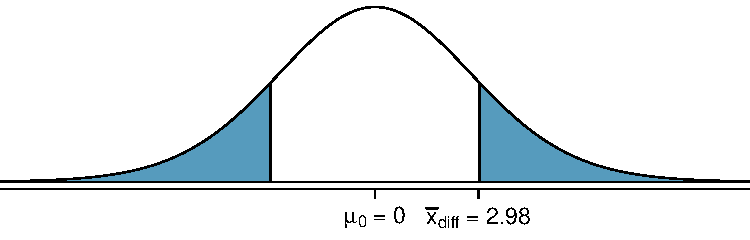
\includegraphics[width=0.65\textwidth]{ch_inference_for_means/figures/textbooksF18/textbooksF18HTTails}
\caption{Sampling distribution for the mean difference in book prices, if the true average difference is zero.}
\label{textbooksF18HTTails}
\end{figure}

\begin{exercisewrap}
\begin{nexercise}
Create a 95\% confidence interval for the average
price difference between books at the UCLA bookstore
and books on Amazon.\footnotemark{}
\end{nexercise}
\end{exercisewrap}
\footnotetext{Conditions
  have already verified and the standard error
  computed in
  Example~\ref{htForDiffInUCLAAndAmazonTextbookPrices}.
  To find the interval,
  identify $t^{\star}_{67}$ using statistical software
  or the $t$-table ($t^{\star}_{67} = 2.00$),
  and plug it, the point estimate,
  and the standard error into the confidence
  interval formula:
  \begin{align*}
  \text{point estimate} \ \pm\ z^{\star} \times SE
      \quad\to\quad
          \uclabookM{} \ \pm\ 2.00 \times \uclabookSE{}
      \quad\to\quad (0.32 6.84)
  \end{align*}
  We are 95\% confident that Amazon is, on average,
  between \$0.32 and \$6.84 less expensive
  than the UCLA Bookstore for UCLA course books.}

\begin{exercisewrap}
\begin{nexercise}
We have strong evidence to conclude Amazon is,
on average, less expensive.
How should this conclusion affect UCLA students'
buying habits?
Should UCLA students always buy their books
on Amazon?\footnotemark{}
\end{nexercise}
\end{exercisewrap}
\footnotetext{The average price difference
  is only mildly useful for this question.
  Examine the distribution shown in
  Figure~\ref{diffInTextbookPricesF18}.
  There are certainly a handful of cases where
  Amazon prices are much below the UCLA Bookstore's,
  which suggests it is worth checking Amazon
  or other online sites before purchasing.
  However, in many cases the Amazon price is
  above what the UCLA Bookstore charges,
  and most of the time the price isn't that different.
  Ultimately, if getting a book immediately from
  the bookstore is notably more convenient,
  e.g. to get started on homework,
  it's likely a good idea to go with the UCLA
  Bookstore unless the price difference on a
  specific book happens to be quite large.

  For reference, this is a very different result
  from what we (the authors) had seen in a similar
  data set from 2010.
  At that time, Amazon prices were almost uniformly
  lower than those of the UCLA Bookstore's and by
  a large margin, making the case to use Amazon over
  the UCLA Bookstore quite compelling at that time.}

\index{data!textbooks|)}
\index{paired data|)}



%__________________
\section{Difference of two means}
\label{differenceOfTwoMeans}

\noindent%
In this section we consider a difference in two population means, $\mu_1 - \mu_2$, under the condition that the data are not paired. Just as with a single sample, we identify conditions to ensure we can use the $t$-distribution with a point estimate of the difference, $\bar{x}_1 - \bar{x}_2$.

We apply these methods in three contexts: determining whether stem cells can improve heart function, exploring the impact of pregnant womens' smoking habits on birth weights of newborns, and exploring whether there is statistically significant evidence that one variation of an exam is harder than another variation. This section is motivated by questions like ``Is there convincing evidence that newborns from mothers who smoke have a different average birth weight than newborns from mothers who don't smoke?''

\subsection{Confidence interval for a difference of means}

\index{data!stem cells, heart function|(}
\index{point estimate!difference of means|(}

Does treatment using embryonic stem cells (ESCs) help improve heart function following a heart attack?
Figure~\ref{summaryStatsForSheepHeartDataWhoReceivedMiceESCs} contains summary statistics for an experiment to test ESCs in sheep that had a heart attack. Each of these sheep was randomly assigned to the ESC or control group, and the change in their hearts' pumping capacity was measured in the study. A~positive value corresponds to increased pumping capacity, which generally suggests a stronger recovery. Our goal will be to identify a 95\% confidence interval for the effect of ESCs on the change in heart pumping capacity relative to the control group.

A point estimate of the difference in the heart pumping variable can be found using the difference in the sample means:
\begin{align*}
\bar{x}_{esc} - \bar{x}_{control}\ =\ 3.50 - (-4.33)\ =\ 7.83
\end{align*}

\begin{figure}[h]
\centering
\begin{tabular}{l rrrrr}
\hline
\hspace{10mm}	& $n$	& $\bar{x}$	& $s$  	 \\
\hline
ESCs		& 9		& 3.50		& 5.17  	\\
control		& 9		& -4.33		& 2.76  	 \\
\hline
\end{tabular}
\caption{Summary statistics of the embryonic stem cell study.}
\label{summaryStatsForSheepHeartDataWhoReceivedMiceESCs}
\end{figure}

%\begin{examplewrap}
%\begin{nexample}{Set up hypotheses that will be used to test whether there is convincing evidence that ESCs actually increase the amount of blood the heart pumps. Also, check conditions for using the $t$-distribution for inference with the point estimate $\bar{x}_1 - \bar{x}_2$. To assist in this assessment, the data are presented in Figure~\ref{stemCellTherapyForHearts}.}\label{exampleToEvaluteWhetherESCsAreHelpfulInImprovingHeartFunctionInSheep}
%We first setup the hypotheses:
%\begin{itemize}
%\setlength{\itemsep}{0mm}
%\item[$H_0$:] The stem cells do not improve heart pumping function. $\mu_{esc} - \mu_{control} = 0$.
%\item[$H_A$:] The stem cells do improve heart pumping function. $\mu_{esc} - \mu_{control} > 0$.
%\end{itemize}
%\end{nexample}
%\end{examplewrap}

\begin{onebox}{Using the $t$-distribution for a difference in means}
\label{ConditionsForTwoSampleTDist}The $t$-distribution can be used for inference when working with the standardized difference of two means if (1) each sample meets the conditions for using the $t$-distribution and (2) the samples are independent.
\end{onebox}

\begin{examplewrap}
\begin{nexample}{Can the $t$-distribution be used to make inference using the point estimate, $\bar{x}_{esc} - \bar{x}_{control} = 7.83$?}
We check the two required conditions:
\begin{enumerate}
\item In this study, the sheep were independent of each other. Additionally, the distributions in Figure~\ref{stemCellTherapyForHearts} don't show any clear deviations from normality, where we watch for prominent outliers in particular for such small samples. These findings imply each sample mean could itself be modeled using a $t$-distribution.
\item The sheep in each group were also independent of each other.
\end{enumerate}
Because both conditions are met, we can use the $t$-distribution to model the difference of the two sample means.
\end{nexample}
\end{examplewrap}

\begin{figure}[h]
\centering
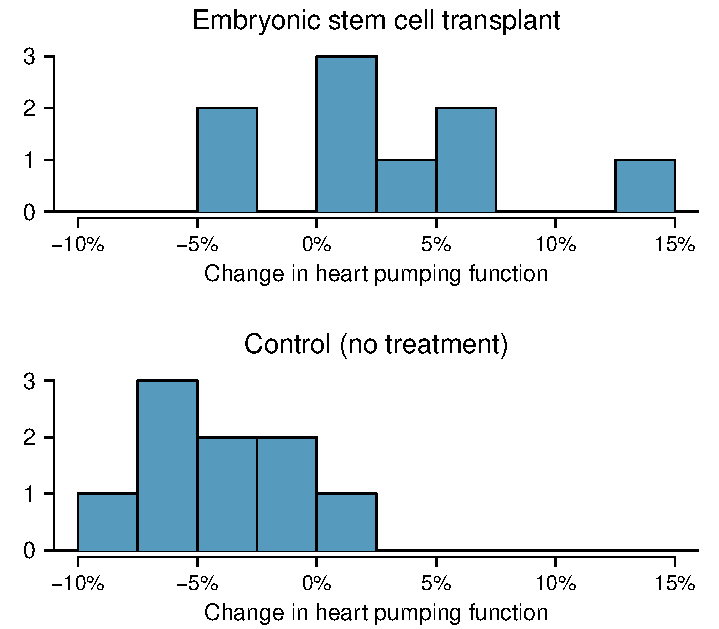
\includegraphics[width=0.58\textwidth]{ch_inference_for_means/figures/stemCellTherapyForHearts/stemCellTherapyForHearts}
\caption{Histograms for both the embryonic stem cell group and the control group. Higher values are associated with greater improvement. We don't see any evidence of skew in these data; however, it is worth noting that skew would be difficult to detect with such a small sample.}
\label{stemCellTherapyForHearts}
\end{figure}

%\begin{onebox}{Conditions for applying the $t$-distribution to $\bar{x}_1 - \bar{x}_2$}
%If the sample means, $\bar{x}_1$ and $\bar{x}_2$, each meet the criteria for using the $t$-distribution and the observations in the two samples are independent, then we can analyze the difference in sample means using the $t$-distribution.
%\end{onebox}

\index{point estimate!difference of means|)}
\index{standard error (SE)!difference in means}

We can quantify the variability in the point estimate, $\bar{x}_{esc} - \bar{x}_{control}$, using the following formula for its standard error:
\index{standard error (SE)!difference in means}
\begin{align*}
SE_{\bar{x}_{esc} - \bar{x}_{control}}
  = \sqrt{\frac{\sigma_{esc}^2}{n_{esc}}
      + \frac{\sigma_{control}^2}{n_{control}}}
\end{align*}
We usually estimate this standard error using standard deviation estimates  based on the samples:
\begin{align*}
SE_{\bar{x}_{esc} - \bar{x}_{control}}
	&= \sqrt{\frac{\sigma_{esc}^2}{n_{esc}} + \frac{\sigma_{control}^2}{n_{control}}} \\
	&\approx \sqrt{\frac{s_{esc}^2}{n_{esc}} + \frac{s_{control}^2}{n_{control}}}
	= \sqrt{\frac{5.17^2}{9} + \frac{2.76^2}{9}} = 1.95
\end{align*}
Because we will use the $t$-distribution, we also must identify the appropriate degrees of freedom. This can be done using computer software. An alternative technique is to use the smaller of $n_1 - 1$ and $n_2 - 1$, which is the method we will typically apply in the examples and guided practice.\footnote{This technique for degrees of freedom is conservative with respect to a Type~1 Error; it is more difficult to reject the null hypothesis using this $df$ method. In this example, computer software would have provided us a more precise degrees of freedom of $df = 12.225$.}

\begin{onebox}{Distribution of a difference of sample means}
The sample difference of two means, $\bar{x}_1 - \bar{x}_2$, can be modeled using the $t$-distribution and the standard error
\begin{align*}
SE_{\bar{x}_{1} - \bar{x}_{2}} = \sqrt{\frac{s_1^2}{n_1} + \frac{s_2^2}{n_2}}
\end{align*}
when each sample mean can itself be modeled using a $t$-distribution and the samples are independent. To calculate the degrees of freedom, use statistical software or the smaller of $n_1 - 1$ and $n_2 - 1$.
\end{onebox}

\begin{examplewrap}
\begin{nexample}{Calculate a 95\% confidence interval for the effect of ESCs on the change in heart pumping capacity of sheep after they've suffered a heart attack.}
We will use the sample difference and the standard error for that point estimate from our earlier calculations:
\begin{align*}
& \bar{x}_{esc} - \bar{x}_{control} = 7.83 \\
& SE = \sqrt{\frac{5.17^2}{9} + \frac{2.76^2}{9}} = 1.95
\end{align*}
Using $df = 8$, we can identify the appropriate $t^{\star}_{df} = t^{\star}_{8}$ for a 95\% confidence interval as 2.31. Finally, we can enter the values into the confidence interval formula:
\begin{align*}
\text{point estimate} \ \pm\ t^{\star} \times SE
  \quad\rightarrow\quad 7.83 \ \pm\ 2.31\times 1.95
  \quad\rightarrow\quad (3.32, 12.34)
\end{align*}
We are 95\% confident that embryonic stem cells improve the heart's pumping function in sheep that have suffered a heart attack by 3.32\% to 12.34\%.
\end{nexample}
\end{examplewrap}

\index{data!stem cells, heart function|)}

\noindent%
As with past statistical inference applications,
there is a well-trodden procedure.
\begin{enumerate}
\item Prepare: retrieve critical contextual information,
    and if appropriate, set up hypotheses.
\item Check: ensure the required conditions are reasonably
    satisfied.
\item Calculate: find the standard error, and then construct
    a confidence interval or find a test statistic and p-value.
\item Conclude: interpret the result in the context of the
    application.
\end{enumerate}
The details change a little from one setting to the next,
but this general approach remain the same.


\subsection{Hypothesis tests based on a difference in means}

\index{data!baby\_smoke|(}

A data set called \data{ncbirths} represents a random sample of 150 cases of mothers and their newborns in North Carolina over a year. Four cases from this data set are represented in Figure~\ref{babySmokeDF}. We are particularly interested in two variables: \var{weight} and \var{smoke}. The \var{weight} variable represents the weights of the newborns and the \var{smoke} variable describes which mothers smoked during pregnancy. We would like to know, is there convincing evidence that newborns from mothers who smoke have a different average birth weight than newborns from mothers who don't smoke? We will use the North Carolina sample to try to answer this question. The smoking group includes 50 cases and the nonsmoking group contains 100 cases, represented in Figure~\ref{babySmokePlotOfTwoGroupsToExamineSkew}.

\begin{figure}[h]
\centering
\begin{tabular}{rrrrrll}
  \hline
 & fAge & mAge & weeks & weight & sexBaby & smoke \\ 
  \hline
1 & NA & 13 &  37 & 5.00 & female & nonsmoker \\ 
  2 & NA & 14 &  36 & 5.88 & female & nonsmoker \\ 
  3 & 19 & 15 &  41 & 8.13 & male & smoker \\ 
  $\vdots$ &   $\vdots$ &   $\vdots$ &   $\vdots$ &   $\vdots$ &   $\vdots$ \\
  150 & 45 & 50 &  36 & 9.25 & female & nonsmoker \\ 
   \hline
\end{tabular}
\caption{Four cases from the \data{ncbirths} data set. The value ``NA'', shown for the first two entries of the first variable, indicates that piece of data is missing.}
\label{babySmokeDF}
\end{figure}

\begin{figure}[hhh]
  \centering
  \Figure{0.63}{babySmokePlotOfTwoGroupsToExamineSkew}
  \caption{The top panel represents birth weights for infants
      whose mothers smoked.
      The bottom panel represents the birth weights for
      infants whose mothers who did not smoke.
      The distributions exhibit moderate-to-strong and
      strong~skew, respectively.%
      \index{skew!example: strong}}
  \label{babySmokePlotOfTwoGroupsToExamineSkew}
\end{figure}

\begin{examplewrap}
\begin{nexample}{Set up appropriate hypotheses to evaluate
    whether there is a relationship between a mother smoking
    and average birth weight.}
  \label{babySmokeHTForWeight}%
  The null hypothesis represents the case of no difference
  between the groups.
  \begin{itemize}
  \setlength{\itemsep}{0mm}
  \item[$H_0$:]
      There is no difference in average birth weight for
      newborns from mothers who did and did not smoke.
      In statistical notation: $\mu_{n} - \mu_{s} = 0$,
      where $\mu_{n}$ represents non-smoking mothers and
      $\mu_s$ represents mothers who smoked.
  \item[$H_A$:]
      There is some difference in average newborn weights
      from mothers who did and did not smoke
      ($\mu_{n} - \mu_{s} \neq 0$).
  \end{itemize}
\end{nexample}
\end{examplewrap}

We check the two conditions necessary to apply the
$t$-distribution to the difference in sample means.
(1)~Because the data come from a simple random sample,
the observations are independent.
Additionally, while each distribution is strongly skewed,
the sample sizes of 50 and 100 would make it reasonable
to model each mean separately using a $t$-distribution.
The skew is reasonable for these sample sizes of 50 and 100.
(2)~The independence reasoning applied in~(1) also ensures
the observations in each sample are independent.
Since both conditions are satisfied, the difference
in sample means may be modeled using a $t$-distribution.

%Summary statistics are shown for each sample in Figure~\ref{SumStatsBirthWeightNewbornsSmoke}.

\begin{figure}[hhh]
\centering
\begin{tabular}{lrr}
	& \resp{smoker} & \resp{nonsmoker} \\
\hline
mean & 6.78 & 7.18 \\
st. dev. & 1.43 & 1.60 \\
samp. size & 50 & 100 \\
\hline
\end{tabular}
\caption{Summary statistics for the \data{ncbirths} data set.}
\label{SumStatsBirthWeightNewbornsSmoke}
\end{figure}

\begin{exercisewrap}
\begin{nexercise}
The summary statistics in
Figure~\ref{SumStatsBirthWeightNewbornsSmoke} may be useful
for this exercise.
\begin{enumerate}[(a)]
\setlength{\itemsep}{0mm}
\item
    What is the point estimate of the population difference,
    $\mu_{n} - \mu_{s}$?
\item
    Compute the standard error of the point estimate from
    part~(a).\footnotemark{}
\end{enumerate}
\end{nexercise}
\end{exercisewrap}
\footnotetext{(a)~The difference in sample means is an
  appropriate point estimate: $\bar{x}_{n} - \bar{x}_{s} = 0.40$.
  (b)~The standard error of the estimate can be estimated using
  the standard error formula:
  \begin{align*}
  SE
    = \sqrt{\frac{\sigma_n^2}{n_n} + \frac{\sigma_s^2}{n_s}}
      \approx \sqrt{\frac{s_n^2}{n_n} + \frac{s_s^2}{n_s}}
    = \sqrt{\frac{1.60^2}{100} + \frac{1.43^2}{50}}
    = 0.26
  \end{align*}}

\begin{examplewrap}
\begin{nexample}{Draw a picture to represent the p-value for
    the hypothesis test from Example~\ref{babySmokeHTForWeight}.}
  \label{pValueForEstOfDiffMeanBirthWeight}%
  To depict the p-value, we draw the distribution of the point
  estimate as though $H_0$ were true and shade areas representing
  at least as much evidence against $H_0$ as what was observed.
  Both tails are shaded because it is a two-sided test.
  \begin{center}
    \Figure{0.6}{distOfDiffOfSampleMeansForBWOfBabySmokeData}
  \end{center}
\end{nexample}
\end{examplewrap}

\begin{examplewrap}
\begin{nexample}{Compute the p-value of the hypothesis
    test using the figure in
    Example~\ref{pValueForEstOfDiffMeanBirthWeight},
    and evaluate the hypotheses using a significance
    level of $\alpha=0.05$.}
  \label{babySmokeHTForWeightComputePValueAndEvalHT}%
  We start by computing the T-score:
  \begin{align*}
  T = \frac{\ 0.40 - 0\ }{0.26} = 1.54
  \end{align*}
  Next, we find the single tail area using software
  (or the table in Appendix~\vref{tDistributionTable}).
  We'll use the
  smaller of $n_n - 1 = 99$ and $n_s - 1 = 49$ as the
  degrees of freedom: $df = 49$.
  The one tail area is 0.065;
  doubling this value gives the two-tail area and p-value,
  0.135.
  This p-value is larger than the significance value, 0.05,
  so we fail to reject the null hypothesis.
  There is insufficient evidence to say there is a difference
  in average birth weight of newborns from North Carolina mothers
  who did smoke during pregnancy and newborns from North Carolina
  mothers who did not smoke during pregnancy.
\end{nexample}
\end{examplewrap}

\begin{exercisewrap}
\begin{nexercise}
We've seen much research suggesting smoking is harmful
during pregnancy, so how could we fail to reject the null
hypothesis in
Example~\ref{babySmokeHTForWeightComputePValueAndEvalHT}?
\footnotemark{}
\end{nexercise}
\end{exercisewrap}
\footnotetext{It is possible that there is some difference
  but we did not detect it.
  If there is a difference, we made a Type~2 Error.
  Notice: we also don't have enough information to,
  if there is an actual difference, confidently say
  which direction that difference would be in.}

\begin{exercisewrap}
\begin{nexercise}
\label{babySmokeHTIDingHowToDetectDifferences}%
If we made a Type~2 Error and there is a difference,
what could we have done differently in data collection
to be more likely to detect the difference?\footnotemark{}
\end{nexercise}
\end{exercisewrap}
\footnotetext{We could have collected more data.
  If the sample sizes are larger, we tend to have
  a better shot at finding a difference if one exists.
  In fact, this is exactly what we would find if we
  examined a larger data set!}

Public service announcement: while we have used this relatively
small data set as an example, larger data sets show that women
who smoke tend to have smaller newborns.
In~fact, some in the tobacco industry actually had the audacity
to tout that as a \emph{benefit} of~smoking:
\begin{quotation}
  \noindent%
  \emph{It's true.
  The babies born from women who smoke are smaller,
  but they're just as healthy as the babies born from
  women who do not smoke.
  And some women would prefer having smaller babies.} \\[2mm]
  \indent\indent\indent\indent\indent\indent%
    - Joseph Cullman, Philip Morris' Chairman of the Board \\
  \indent\indent\indent\indent\indent\indent%
  {\color{white}...}on CBS' \emph{Face the Nation}, Jan 3,~1971
\end{quotation}
Fact check: the babies from women who smoke are not actually
as healthy as the babies from women who do not
smoke.\footnote{You can watch an episode of John Oliver
  on \emph{Last Week Tonight} to explore the present day
  offenses of the tobacco industry.
  Please be aware that there is some adult language:
  \oiRedirect{textbook-johnoliver_tobacco}{youtu.be/6UsHHOCH4q8}.}
% Resource on this topic:
% http://archive.tobacco.org/Documents/documentquotes.html

\index{data!baby\_smoke|)}


\subsection{Case study: two versions of a course exam}

\index{data!two exam comparison|(}

An instructor decided to run two slight variations of the same exam. Prior to passing out the exams, she shuffled the exams together to ensure each student received a random version. Summary statistics for how students performed on these two exams are shown in Figure~\ref{summaryStatsForTwoVersionsOfExams}. Anticipating complaints from students who took Version~B, she would like to evaluate whether the difference observed in the groups is so large that it provides convincing evidence that Version~B was more difficult (on average) than Version~A.

\begin{figure}[hht]
\centering
\begin{tabular}{l rrrrr}
\hline
Version\hspace{2mm}	& $n$	& $\bar{x}$	& $s$	& min	& max  \\
\hline
A		& 30		& 79.4		& 14 	& 45		& 100 \\
B		& 27		& 74.1		& 20		& 32		& 100 \\
\hline
\end{tabular}
\caption{Summary statistics of scores for each exam version.}
\label{summaryStatsForTwoVersionsOfExams}
\end{figure}

\begin{exercisewrap}
\begin{nexercise}
\label{htSetupForEvaluatingTwoExamVersions}%
Construct a hypotheses to evaluate whether the observed
difference in sample means, $\bar{x}_A - \bar{x}_B=5.3$,
is due to chance. We will later evaluate these hypotheses
using $\alpha = 0.01$.\footnotemark{}
\end{nexercise}
\end{exercisewrap}
\footnotetext{Because the teacher did not expect one exam to be more difficult prior to examining the test results, she should use a two-sided hypothesis test. $H_0$: the exams are equally difficult, on average. $\mu_A - \mu_B = 0$. $H_A$: one exam was more difficult than the other, on average. $\mu_A - \mu_B \neq 0$.}

\begin{exercisewrap}
\begin{nexercise} \label{conditionsForTDistForEvaluatingTwoExamVersions}%
To evaluate the hypotheses in Guided Practice~\ref{htSetupForEvaluatingTwoExamVersions} using the $t$-distribution, we must first verify assumptions.\footnotemark{}
\begin{enumerate}[(a)]
\setlength{\itemsep}{0mm}
\item
    Does it seem reasonable that the scores are independent
    within each group?
\item
    What about the normality / skew condition for observations
    in each group?
\item
    Do you think scores from the two groups would be independent
    of each other, i.e. the two samples are
    independent?
\end{enumerate}
\end{nexercise}
\end{exercisewrap}
\footnotetext{(a) It is probably reasonable to conclude the scores are independent, provided there was no cheating. (b) The summary statistics suggest the data are roughly symmetric about the mean, and it doesn't seem unreasonable to suggest the data might be normal. Note that since these samples are each nearing 30, moderate skew in the data would be acceptable. (c) It seems reasonable to suppose that the samples are independent since the exams were handed out randomly.}

After verifying the conditions for each sample and confirming the samples are independent of each other, we are ready to conduct the test using the $t$-distribution. In this case, we are estimating the true difference in average test scores using the sample data, so the point estimate is $\bar{x}_A - \bar{x}_B = 5.3$. The standard error of the estimate can be calculated~as
\begin{align*}
SE
  = \sqrt{\frac{s_A^2}{n_A} + \frac{s_B^2}{n_B}}
  = \sqrt{\frac{14^2}{30} + \frac{20^2}{27}}
  = 4.62
\end{align*}
Finally, we construct the test statistic:
\begin{align*}
T
  = \frac{\text{point estimate} - \text{null value}}{SE}
  = \frac{(79.4-74.1) - 0}{4.62}
  = 1.15
\end{align*}
If we have a computer handy, we can identify the degrees
of freedom as 45.97.
Otherwise we use the smaller of $n_1-1$ and $n_2-1$: $df=26$. 

\begin{figure}[h]
  \centering
  \Figure{0.63}{pValueOfTwoTailAreaOfExamVersionsWhereDFIs26}
  \caption{The $t$-distribution with 26 degrees of freedom.
      The shaded right tail represents values with $T \geq 1.15$.
      Because it is a two-sided test, we also shade the
      corresponding lower tail.}
  \label{pValueOfTwoTailAreaOfExamVersionsWhereDFIs26}
\end{figure}

\begin{examplewrap}
\begin{nexample}{Identify the p-value using $df = 26$
    and provide a conclusion in the context of the case study.}
  Using software, we can find the one-tail area (0.13)
  and then double this value to get the two-tail area,
  which is the p-value: 0.26.
  (Alternatively, we could use the $t$-table in
  Appendix~\ref{tDistributionTable}.)
  We examine row $df=26$ in the $t$-table.
  In Guided Practice~\ref{},
  we specified that we would use $\alpha = 0.01$.
  Since the p-value is larger than $\alpha$,
  we do not reject the null hypothesis.
  That is, the data do not convincingly show that one exam
  version is more difficult than the other, and the teacher
  should not be convinced that she should add points to the
  Version~B exam scores.
\end{nexample}
\end{examplewrap}

\index{data!two exam comparison|)}

%\subsection{Summary for inference using the $t$-distribution}
%
%\Comment{This subsection should be heavily updated.}
%
%%When considering the difference of two means, there are two common cases: the two samples are paired or they are independent. (There are instances where the data are neither paired nor independent, e.g. see blocking in Section~\ref{experimentalDesignPrinciples}.) The paired case was treated in Section~\ref{pairedData}, where the one-sample methods were applied to the differences from the paired observations. We examined the second and more complex scenario in this section.
%
%\textbf{Hypothesis tests.} When applying the $t$-distribution for a hypothesis test, we proceed as follows:
%\begin{itemize}
%\setlength{\itemsep}{0mm}
%\item Write appropriate hypotheses.
%\item Verify conditions for using the $t$-distribution.
%\begin{itemize}
%\item One-sample or differences from paired data: the observations (or differences) must be independent and nearly normal. For larger sample sizes, we can relax the nearly normal requirement, e.g. slight skew is okay for sample sizes of 15, moderate skew for sample sizes of 30, and strong skew for sample sizes of 60.
%\item For a difference of means when the data are not paired: each sample mean must separately satisfy the one-sample conditions for the $t$-distribution, and the data in the groups must also be independent.
%\end{itemize}
%\item Compute the point estimate of interest, the standard error, and the degrees of freedom. For $df$, use $n-1$ for one sample, and for two samples use either statistical software or the smaller of $n_1 - 1$ and $n_2 - 1$.
%\item Compute the T-score and p-value.
%\item Make a conclusion based on the p-value, and write a conclusion in context and in plain language so anyone can understand the result.
%\end{itemize}
%\noindent\textbf{Confidence intervals.} Similarly, the following is how we generally computed a confidence interval using a $t$-distribution:
%\begin{itemize}
%\item Verify conditions for using the $t$-distribution. (See above.)
%\item Compute the point estimate of interest, the standard error, the degrees of freedom, and $t^{\star}_{df}$.
%\item Calculate the confidence interval using the general formula, point estimate $\pm\ t_{df}^{\star} SE$.
%\item Put the conclusions in context and in plain language so even non-data scientists can understand the results.
%\end{itemize}
%
%\CalculatorVideos{confidence intervals and hypothesis tests for a difference of means}


%\subsection{Examining the standard error formula (special topic)}
%
%The formula for the standard error of the difference in two means is similar to the formula for other standard errors. Recall that the standard error of a single mean, $\bar{x}_1$, can be approximated by
%\begin{align*}
%SE_{\bar{x}_1} = \frac{s_1}{\ \sqrt{n_1}\ }
%\end{align*}
%where $s_1$ and $n_1$ represent the sample standard deviation and sample size.
%
%The standard error of the difference of two sample means can be constructed from the standard errors of the separate sample means:
%\begin{align*}
%SE_{\bar{x}_{1} - \bar{x}_{2}}
%	= \sqrt{SE_{\bar{x}_1}^2 + SE_{\bar{x}_2}^2}
%	= \sqrt{\frac{s_1^2}{{n_1}} + \frac{s_2^2}{{n_2}}}
%\end{align*}
%This special relationship follows from probability theory.
%
%\begin{exercisewrap}
%\begin{nexercise}
%\label{derivingSEForDiffOfTwoMeansExercise}%
%Prerequisite: Section~\ref{randomVariablesSection}.
%We can rewrite the equation above in a different way:
%\begin{align*}
%SE_{\bar{x}_{1} - \bar{x}_{2}}^2
%  = SE_{\bar{x}_1}^2 + SE_{\bar{x}_2}^2
%\end{align*}
%Explain where this formula comes from using the ideas of probability theory.\footnotemark{}
%\end{nexercise}
%\end{exercisewrap}
%\footnotetext{The standard error squared represents the variance of the estimate. If $X$ and $Y$ are two random variables with variances $\sigma_x^2$ and $\sigma_y^2$, then the variance of $X-Y$ is $\sigma_x^2 + \sigma_y^2$. Likewise, the variance corresponding to $\bar{x}_1 - \bar{x}_2$ is $\sigma_{\bar{x}_1}^2 + \sigma_{\bar{x}_2}^2$. Because $\sigma_{\bar{x}_1}^2$ and $\sigma_{\bar{x}_2}^2$ are just another way of writing $SE_{\bar{x}_1}^2$ and  $SE_{\bar{x}_2}^2$, the variance associated with $\bar{x}_1 - \bar{x}_2$ may be written as $SE_{\bar{x}_1}^2 + SE_{\bar{x}_2}^2$.}


\subsection{Pooled standard deviation estimate (special topic)}
\label{pooledStandardDeviations}

Occasionally, two populations will have standard deviations that are so similar that they can be treated as identical. For example, historical data or a well-understood biological mechanism may justify this strong assumption. In such cases, we can make the $t$-distribution approach slightly more precise by using a pooled standard deviation.

The \term{pooled standard deviation} of two groups is a way to use data from both samples to better estimate the standard deviation and standard error. If $s_1^{}$ and $s_2^{}$ are the standard deviations of groups 1 and 2 and there are good reasons to believe that the population standard deviations are equal, then we can obtain an improved estimate of the group variances by pooling their data:
\begin{align*}
s_{pooled}^2 = \frac{s_1^2\times (n_1-1) + s_2^2\times (n_2-1)}{n_1 + n_2 - 2}
\end{align*}
where $n_1$ and $n_2$ are the sample sizes, as before. To use this new statistic, we substitute $s_{pooled}^2$ in place of $s_1^2$ and $s_2^2$ in the standard error formula, and we use an updated formula for the degrees of freedom:
\begin{align*}
df = n_1 + n_2 - 2
\end{align*}

The benefits of pooling the standard deviation are realized through obtaining a better estimate of the standard deviation for each group and using a larger degrees of freedom parameter for the $t$-distribution. Both of these changes may permit a more accurate model of the sampling distribution of $\bar{x}_1 - \bar{x}_2$, if the standard deviations of the two groups are~equal.

\begin{onebox}
    {Pool standard deviations only after careful consideration}
  A pooled standard deviation is only appropriate when
  background research indicates the population standard
  deviations are nearly equal.
  When the sample size is large and the condition
  may be adequately checked with data, the benefits
  of pooling the standard deviations greatly diminishes.
\end{onebox}



%__________________
\section{Power calculations for a difference of means}
\label{PowerForDifferenceOfTwoMeans}

\noindent%
Often times in experiment planning, there are two competing considerations:
\begin{itemize}
\setlength{\itemsep}{0mm}
\item We want to collect enough data that we can detect important effects.
\item Collecting data can be expensive, and in experiments involving people, there may be some risk to patients.
\end{itemize}
In this section, we focus on the context of a clinical trial, which is a health-related experiment where the subject are people, and we will determine an appropriate sample size where we can be 80\% sure that we would detect any practically important effects.\footnote{Even though we don't cover it explicitly, similar sample size planning is also helpful for observational studies.}


\subsection{Going through the motions of a test}

We're going to go through the motions of a hypothesis test. This will help us frame our calculations for determining an appropriate sample size for the study.

\begin{examplewrap}
\begin{nexample}{Suppose a pharmaceutical company has developed
    a new drug for lowering blood pressure, and they are
    preparing a clinical trial (experiment) to test the
    drug's effectiveness.
    They recruit people who are taking a particular standard
    blood pressure medication.
    People in the control group will continue to take their
    current medication through generic-looking pills to ensure
    blinding.
    Write down the hypotheses for a two-sided hypothesis test
    in this context.}
  Generally, clinical trials use a two-sided alternative
  hypothesis, so below are suitable hypotheses for this context:
  \begin{description}
  \setlength{\itemsep}{0mm}
  \item[$H_0$:]
      The new drug performs exactly as well as the
      standard medication. \\
      $\mu_{trmt} - \mu_{ctrl} = 0$.
  \item[$H_A$:]
      The new drug's performance differs from the
      standard medication. \\
      $\mu_{trmt} - \mu_{ctrl} \neq 0$.
  \end{description}
%  This two-sided test ensures we'll be alerted if either
%  the new drug works better or worse than the standard
%  medication.
\end{nexample}
\end{examplewrap}

\begin{examplewrap}
\begin{nexample}{The researchers would like to run the clinical
    trial on patients with systolic blood pressures between 140
    and 180~mmHg.
    Suppose previously published studies suggest that the
    standard deviation of the patients' blood pressures will
    be about 12~mmHg and the distribution of patient blood
    pressures will be approximately symmetric.\footnotemark{}
    If~we had 100 patients per group, what would be the
    approximate standard error for
    $\bar{x}_{trmt} - \bar{x}_{ctrl}$?}
  The standard error is calculated as follows:
  \begin{align*}
  SE_{\bar{x}_{trmt} - \bar{x}_{ctrl}}
    = \sqrt{\frac{s_{trmt}^2}{n_{trmt}} +
        \frac{s_{ctrl}^2}{n_{ctrl}}}
    = \sqrt{\frac{12^2}{100} + \frac{12^2}{100}}
    = 1.70
  \end{align*}
  This may be an imperfect estimate of
  $SE_{\bar{x}_{trmt} - \bar{x}_{ctrl}}$,
  since the standard deviation estimate we used may not
  be perfectly correct for this group of patients.
  However, it is sufficient for our purposes.
\end{nexample}
\end{examplewrap}
\footnotetext{In this particular study, we'd generally measure
  each patient's blood pressure at the beginning and end
  of the study, and then the outcome measurement for
  the study would be the average change in blood pressure.
  That is, both $\mu_{trmt}$ and $\mu_{ctrl}$ would
  represent average differences.
  This is what you might think of as a 2-sample paired
  testing structure, and we'd analyze it exactly just like
  a hypothesis test for a difference in the average change
  for patients.
  In the calculations we perform here, we'll suppose
  that 12~mmHg is the predicted standard deviation of
  a patient's blood pressure difference over the course
  of the study.}

\begin{examplewrap}
\begin{nexample}{What does the null distribution of
    $\bar{x}_{trmt} - \bar{x}_{ctrl}$ look like?}
  The degrees of freedom are greater than 30, so the
  distribution of $\bar{x}_{trmt} - \bar{x}_{ctrl}$
  will be approximately normal.
  The standard deviation of this distribution
  (the standard error) would be about 1.70, and under
  the null hypothesis, its mean would be 0.
  \begin{center}
  \Figures{0.93}{power_null_0_1-7}{power_null_A_0_1-7}
  \end{center}
\end{nexample}
\end{examplewrap}

\begin{examplewrap}
\begin{nexample}{For what values of
    $\bar{x}_{trmt} - \bar{x}_{ctrl}$ would we reject
    the null hypothesis?}
  For $\alpha = 0.05$, we would reject $H_0$ if the difference
  is in the lower 2.5\% or upper 2.5\% tail:
  \begin{description}
  \setlength{\itemsep}{0mm}
  \item[Lower 2.5\%:]
      For the normal model, this is 1.96 standard errors
      below~0, so any difference smaller than
      $-1.96 \times 1.70 = -3.332$~mmHg.
  \item[Upper 2.5\%:]
      For the normal model, this is 1.96 standard errors
      above~0, so any difference larger than
      $1.96 \times 1.70 = 3.332$~mmHg.
  \end{description}
  The boundaries of these \term{rejection regions} are shown below:
  \begin{center}
  \Figures{0.93}{power_null_0_1-7}
      {power_null_B_0_1-7_with_rejection_region}
  \end{center}
\end{nexample}
\end{examplewrap}

Next, we'll perform some hypothetical calculations to determine
the probability we reject the null hypothesis, if the alternative
hypothesis were actually true.


\subsection%[Computing the power for a 2-sample test]
    {Computing the power for a 2-sample test}

When planning a study, we want to know how likely we are
to detect an effect we care about.
In~other words, if there is a real effect, and that effect
is large enough that it has practical value, then what's
the probability that we detect that effect?
This probability is called the \term{power}, and we can
compute it for different sample sizes or for different
\emph{effect sizes}.

We first determine what is a practically significant result.
Suppose that the company researchers care about finding any
effect on blood pressure that is 3~mmHg or larger vs the
standard medication.
Here, 3~mmHg is the minimum \term{effect size} of interest,
and we want to know how likely we are to detect this size
of an effect in the study.

\begin{examplewrap}
\begin{nexample}{Suppose we decided to move forward with
    100 patients per treatment group and the new drug reduces
    blood pressure by an additional 3~mmHg relative to the
    standard medication.
    What is the probability that we detect a drop?}
  \label{PowerFor100AtNeg3}%
  Before we even do any calculations, notice that if
  $\bar{x}_{trmt} - \bar{x}_{ctrl} = -3$~mmHg, there
  wouldn't even be sufficient evidence to reject $H_0$.
  That's not a good sign.

  To calculate the probability that we will reject $H_0$,
  we need to determine a few things:
  \begin{itemize}
  \setlength{\itemsep}{0mm}
  \item
      The sampling distribution for
      $\bar{x}_{trmt} - \bar{x}_{ctrl}$ when the true difference
      is -3~mmHg.
      This is the same as the null distribution,
      except it is shifted to the left by~3:
      \begin{center}
      \Figures{0.87}{power_null_0_1-7}
          {power_null_C_0_1-7_with_alt_at_3}
      \end{center}
  \item
      The rejection regions, which are outside of the
      dotted lines above.
  \item
      The fraction of the distribution that falls in the
      rejection region.
  \end{itemize}
  In short, we need to calculate the probability that
  $x < -3.332$ for a normal distribution with mean -3
  and standard deviation~1.7.
  To do so, we first shade the area we want to calculate:
  \begin{center}
    \Figures{0.93}{power_null_0_1-7}
        {power_null_D_0_1-7_with_alt_at_3_and_shaded}
  \end{center}
  We'll use a normal approximation, which is good approximation
  when the degrees of freedom is about 30 or more.
  We'll start by calculating the Z-score and find the tail area
  using either statistical software or the probability table:
  \begin{align*}
  Z = \frac{-3.332 - (-3)}{1.7} = -0.20 \qquad \to \qquad 0.42
  \end{align*}
  The power for the test is about 42\% when
  $\mu_{trmt} - \mu_{ctrl} = -3$ and each group has
  a sample size of~100.
\end{nexample}
\end{examplewrap}

In Example~\ref{PowerFor100AtNeg3}, we ignored the upper
rejection region in the calculation, which was in the
opposite direction of the hypothetical truth, i.e. -3.
The reasoning?
There wouldn't be any value in rejecting the null hypothesis
and concluding there was an increase when in fact there was
a decrease.

We've also been applying the normal distribution instead
of the $t$-distribution.
This is a convenience, and if the sample size is too small,
we'd need to revert back to using the $t$-distribution.
We'll discuss this a bit further at the end of this section.



\subsection{Determining a proper sample size}

In the last example, we found that if we have a sample size
of 100 in each group, we can only detect an effect size of
3~mmHg with a probability of about 0.42.
Suppose the researchers moved forward and only used
100 patients per group, and the data did not support
the alternative hypothesis,
i.e. the researchers did not reject $H_0$.
This is a very bad situation to be in for a few reasons:
\begin{itemize}
\setlength{\itemsep}{0mm}
\item
    In the back of the researchers' minds, they'd all be
    wondering, \emph{maybe there is a real and meaningful
    difference, but we weren't able to detect it with such
    a small sample}. 
\item
    The company probably invested hundreds of millions
    of dollars in developing the new drug, so now they
    are left with great uncertainty about its potential
    since the experiment didn't have a great shot at
    detecting effects that could still be important.
\item
    Patients were subjected to the drug, and we can't even
    say with much certainty that the drug doesn't help
    (or harm) patients.
\item
    Another clinical trial may need to be run to get a more
    conclusive answer as to whether the drug does hold any
    practical value, and conducting a second clinical trial
    may take years and many millions of dollars.
\end{itemize}
We want to avoid this situation, so we need to determine
an appropriate sample size to ensure we can be pretty
confident that we'll detect any effects that are practically
important.
As mentioned earlier, a change of 3~mmHg was deemed to be the
minimum difference that was practically important.
As~a first step, we could calculate power for several
different sample sizes.
For instance, let's try 500 patients per group.

\begin{exercisewrap}
\begin{nexercise}
Calculate the power to detect a change of -3~mmHg when using
a sample size of 500 per group.\footnotemark{}
\begin{enumerate}[(a)]
\setlength{\itemsep}{0mm}
\item
    Determine the standard error (recall that the standard
    deviation for patients was expected to be about 12~mmHg).
\item
    Identify the null distribution and rejection regions.
\item
    Identify the alternative distribution when
    $\mu_{trmt} - \mu_{ctrl} = -3$.
\item
    Compute the probability we reject the null hypothesis.
\end{enumerate}
\end{nexercise}
\end{exercisewrap}
\footnotetext{(a) The standard error is given as
  $SE = \sqrt{\frac{12^2}{500} + \frac{12^2}{500}} = 0.76$.\\
  (b)~\&~(c)~The null distribution, rejection boundaries,
  and alternative distribution are shown below: \\
  \indent%
  \Figures{0.7}{power_null_0_0-76}
      {power_null_0_0-76_with_alt_at_3_and_shaded} \\
  The rejection regions are the areas on the outside of the
  two dotted lines and are at $\pm 0.76 \times 1.96 = \pm 1.49$. \\
  (d)~The area of the alternative distribution where
  $\mu_{trmt} - \mu_{ctrl} = -3$ has been shaded.
  We compute the Z-score and find the tail area:
  $Z = \frac{-1.49 - (-3)}{0.76} = 1.99 \to 0.977$.
%  (can use $df = 500$ from the minimum of the two sample
%  sizes minus 1),
%  which is the power of the test for a difference of 3~mmHg.
  With 500 patients per group, we would be about 97.7\% sure
  (or~more) that we'd detect any effects that are at least
  3~mmHg in size.}

The researchers decided 3~mmHg was the minimum difference
that was practically important, and with a sample size of~500,
we can be very certain (97.7\% or better) that we will detect
any such difference.
We now have moved to another extreme where we are exposing
an unnecessary number of patients to the new drug in the
clinical trial.
Not only is this ethically questionable, but it would also
cost a lot more money than is necessary to be quite sure
we'd detect any important effects.

The most common practice is to identify the sample size where
the power is around 80\%, and sometimes 90\%.
Other values may be reasonable for a specific context,
but 80\% and 90\% are most commonly targeted as a good
balance between high power and not exposing too many
patients to a new treatment (or wasting too much money).

We could compute the power of the test at several other
possible sample sizes until we find one that's close to~80\%,
but there's a better way.
We should solve the problem backwards.

\begin{examplewrap}
\begin{nexample}{What sample size will lead to a power of 80\%?}
  We'll assume we have a large enough sample that the normal
  distribution is a good approximation for the test statistic,
  since the normal distribution and the $t$-distribution
  look almost identical when the degrees of freedom are
  moderately large (e.g. $df \geq 30$).
  If that doesn't turn out to be true, then we'd need to make
  a correction.

  We start by identifying the Z-score that would give us a lower
  tail of 80\%.
  For a moderately large sample size per group,
  the Z-score for a lower tail of 80\% would be about $Z = 0.84$.
%  (If our calculations suggest a very sample size,
%  we should recalculate this part and basically do the
%  problem one more time.)
  \begin{center}
    \Figure{0.93}{power_best_sample_size}
  \end{center}
  Additionally, the rejection region extends
  $1.96\times SE$ from the center of the null distribution
  for $\alpha = 0.05$.
  This allows us to calculate the target distance between
  the center of the null and alternative distributions in
  terms of the standard error:
  \begin{align*}
  0.84 \times SE + 1.96 \times SE = 2.8 \times SE
  \end{align*}
  In our example, we want the distance between the null
  and alternative distributions' centers to equal the minimum
  effect size of interest, 3~mmHg, which allows us to set up
  an equation between this difference and the standard error:
  \begin{align*}
  3 &= 2.8 \times SE \\
  3 &= 2.8 \times \sqrt{\frac{12^2}{n} + \frac{12^2}{n}} \\
  n &= \frac{2.8^2}{3^2} \times \left( 12^2 + 12^2 \right)
    = 250.88 \\
  \end{align*}
  We should target about 251 patients per group.

  Had the suggested sample size been relatively small
  -- roughly 30 or smaller -- it would have been a good idea
  to rework the calculations using the degrees of fredom
  for the smaller sample size under that initial sample size.
  That is, we would have revised the 0.84 and 1.96
  values based on degrees of freedom implied by the initial
  sample size.
  The revised sample size target would generally have then
  been a little larger.
\end{nexample}
\end{examplewrap}

The standard error difference of $2.8 \times SE$ is specific
to a context where the targeted power is 80\% and the
significance level is $\alpha = 0.05$.
If the targeted power is 90\% or if we use a different
significance level, then we'll use something a little
different than $2.8 \times SE$.

%\begin{examplewrap}
%\begin{nexample}{Suppose the suggested sample size from
%    the power calculation was 15 per group.
%    This is a relatively small sample size,
%    and the assumptions about the sample size being
%    large in Example~\ref{}
%    wouldn't be valid.
%    What should we do?}
%  First, recognizing that there is \emph{something}
%  to do is already great here:
%  it's easy to forget the earlier assumption about
%  a moderately large sample size.
%  So if you catch yourself here, that is something
%  to be commended!
%
%  Next, we basically update the values of 0.84 and 1.96
%  in the calculations.
%  First, we identify the degrees of freedom
%  ($df = 14$ as a rough guide, though 
%  We'd find the values
%  corresponding to this more precise $t$-distribution.
%  For example, had the sample-size per group been suggested
%  as~15, we would have used $df = 14$;
%  this would have led to a T-score of 0.87 (in place of 0.84)
%  and a rejection region cutoff of 2.14.
%  The reworked sample size would then have been suggested
%  as about 16\% larger.
%  If we did not do this extra step, our estimated power would
%  drop from 80\% to 74\%.
%  While that would not be the end of the world, being precise
%  is part of the job of being a data scientist!
%\end{nexample}
%\end{examplewrap}

\begin{exercisewrap}
\begin{nexercise}
Suppose the targeted power was 90\% and we were using
$\alpha = 0.01$.
How many standard errors should separate the centers
of the null and alternative distribution, where the
alternative distribution is centered at the minimum
effect size of interest?\footnotemark{}
\end{nexercise}
\end{exercisewrap}
\footnotetext{First, find the Z-score such that 90\% of the
  distribution is below it: $Z = 1.28$.
  Next, find the cutoffs for the rejection regions: $\pm 2.58$.
  Then the difference in centers should be about
  $1.28 \times SE + 2.58 \times SE = 3.86 \times SE$.}

\begin{exercisewrap}
\begin{nexercise}
What are some considerations that are important in determining
what the power should be for an experiment?\footnotemark{}
\end{nexercise}
\end{exercisewrap}
\footnotetext{Answers will vary, but here are a few
  important considerations:
  \begin{itemize}
  \setlength{\itemsep}{0mm}
  \item Whether there is any risk to patients in the study.
  \item The cost of enrolling more patients.
  \item The potential downside of not detecting an effect
      of interest.
  \end{itemize}}

Figure~\ref{power_curve_neg-3} shows the power for sample sizes from 20~patients to 5,000~patients when $\alpha = 0.05$ and the true difference is -3. This curve was constructed by writing a program to compute the power for many different sample sizes.

\begin{figure}[h]
  \centering
  \Figures{0.9}{power_curve}{power_curve_neg-3}
  \caption{The curve shows the power for different sample
      sizes in the context of the blood pressure example when
      the true difference is~-3.
      Having more than about 250 to 350 observations doesn't
      provide much additional value in detecting an effect when
      $\alpha = 0.05$.}
  \label{power_curve_neg-3}
\end{figure}

%\begin{exercisewrap}
%\begin{nexercise}
%
%\end{nexercise}
%\end{exercisewrap}

Power calculations for expensive or risky experiments are
critical.
However, what about experiments that are inexpensive and
where the ethical considerations are minimal?
For example, if we are doing final testing on a new feature
on a popular website, how would our sample size considerations
change?
As before, we'd want to make sure the sample is big enough.
However, suppose the feature has undergone some testing and
is known to perform well
(e.g.~the website's users seem to enjoy the feature).
Then it may be reasonable to run a larger experiment
if there's value from having a more precise estimate
of the feature's effect, such as helping guide the
development of the next useful feature.




%__________________
\section{Comparing many means with ANOVA}
\label{anovaAndRegrWithCategoricalVariables}

\index{analysis of variance (ANOVA)|(}

\noindent%
Sometimes we want to compare means across many groups. We might initially think to do pairwise comparisons; for example, if there were three groups, we might be tempted to compare the first mean with the second, then with the third, and then finally compare the second and third means for a total of three comparisons. However, this strategy can be treacherous. If we have many groups and do many comparisons, it is likely that we will eventually find a difference just by chance, even if there is no difference in the populations.

In this section, we will learn a new method called \term{analysis of variance (ANOVA)} and a new test statistic called $F$. ANOVA uses a single hypothesis test to check whether the means across many groups are equal:
\begin{itemize}
\setlength{\itemsep}{0mm}
\item[$H_0$:] The mean outcome is the same across all groups. In statistical notation, $\mu_1 = \mu_2 = \cdots = \mu_k$ where $\mu_i$ represents the mean of the outcome for observations in category $i$.
\item[$H_A$:] At least one mean is different.
\end{itemize}
Generally we must check three conditions on the data before performing ANOVA:
\begin{itemize}
\setlength{\itemsep}{0mm}
\item the observations are independent within and across groups,
\item the data within each group are nearly normal, and
\item the variability across the groups is about equal.
\end{itemize}
When these three conditions are met, we may perform an ANOVA to determine whether the data provide strong evidence against the null hypothesis that all the $\mu_i$ are equal.

\begin{examplewrap}
\begin{nexample}{College departments commonly run multiple lectures of the same introductory course each semester because of high demand. Consider a statistics department that runs three lectures of an introductory statistics course. We might like to determine whether there are statistically significant differences in first exam scores in these three classes ($A$, $B$, and $C$). Describe appropriate hypotheses to determine whether there are any differences between the three classes.} \label{firstExampleForThreeStatisticsClassesAndANOVA}
The hypotheses may be written in the following form:
\begin{itemize}
\setlength{\itemsep}{0mm}
\item[$H_0$:] The average score is identical in all lectures. Any observed difference is due to chance. Notationally, we write $\mu_A=\mu_B=\mu_C$.
\item[$H_A$:] The average score varies by class. We would reject the null hypothesis in favor of the alternative hypothesis if there were larger differences among the class averages than what we might expect from chance alone.
\end{itemize}
\end{nexample}
\end{examplewrap}

Strong evidence favoring the alternative hypothesis in ANOVA is described by unusually large differences among the group means. We will soon learn that assessing the variability of the group means relative to the variability among individual observations within each group is key to ANOVA's success.

\begin{examplewrap}
\begin{nexample}{Examine Figure~\ref{toyANOVA}. Compare groups I, II, and III. Can you visually determine if the differences in the group centers is due to chance or not? Now compare groups IV, V, and VI. Do these differences appear to be due to chance?}

Any real difference in the means of groups I, II, and III is difficult to discern, because the data within each group are very volatile relative to any differences in the average outcome. On the other hand, it appears there are differences in the centers of groups IV, V, and VI. For instance, group V appears to have a higher mean than that of the other two groups. Investigating groups IV, V, and VI, we see the differences in the groups' centers are noticeable because those differences are large \emph{relative to the variability in the individual observations within each group}.
\end{nexample}
\end{examplewrap}

\begin{figure}[h]
  \centering
  \Figure{0.68}{toyANOVA}
  \caption{Side-by-side dot plot for the outcomes for six groups.}
  \label{toyANOVA}
\end{figure}


\subsection{Is batting performance related to player position in MLB?}

\index{data!MLB batting|(}

\newcommand{\mlbdata}{\data{bat18}}
\newcommand{\mlbN}{429}
\newcommand{\mlbK}{3}
\newcommand{\mlbMinAB}{100}
\newcommand{\mlbDFA}{2}
\newcommand{\mlbDFB}{426}
\newcommand{\mlbF}{5.077}
\newcommand{\mlbPvalue}{0.0066}

We would like to discern whether there are real differences
between the batting performance of baseball players according
to their position:
outfielder (\resp{OF}), infielder (\resp{IF}),
%designated hitter (\resp{DH}),
and catcher (\resp{C}).
We will use a data set called \mlbdata{},
which includes batting records of \mlbN{} Major League
Baseball (MLB) players from the 2018 season who had
at least \mlbMinAB{} at bats.
Six of the \mlbN{} cases represented in \mlbdata{}
are shown in Figure~\ref{mlbBat18DataMatrix},
and descriptions for each variable are provided
in Figure~\ref{mlbBat18Variables}.
The measure we will use for the player batting
performance (the outcome variable) is on-base
percentage (\var{OBP}).
The on-base percentage roughly represents the fraction
of the time a player successfully gets on base or hits
a home run.

\begin{figure}[h]
\centering
\begin{tabular}{r lll ccc ccc}
  \hline
  & name & team & position & AB & H & HR &RBI & AVG & OBP \\ 
  \hline
  1 &  Abreu, J & CWS & IF &  499 &  132 &   22 &
      78 & 0.265 & 0.325 \\
  2 &  Acuna Jr., R & ATL & OF &  433 &  127 &   26 &
      64 & 0.293 & 0.366 \\
  3 &  Adames, W & TB & IF &  288 &   80 &   10 &
      34 & 0.278 & 0.348 \\
  $\vdots$ & $\vdots$ & $\vdots$ & $\vdots$ & $\vdots$ &
      $\vdots$ & $\vdots$ & $\vdots$ \\
  427 &  Zimmerman, R & WSH & IF & 288 &   76 &
      13 &   51 & 0.264 & 0.337 \\
  428 &  Zobrist, B & CHC & IF &  455 &  139 &    9 &   58 & 0.305 & 0.378 \\
  \mlbN{} &  Zunino, M & SEA & C &  373 &   75 &   20 &
      44 & 0.201 & 0.259 \\
   \hline
\end{tabular}
\caption{Six cases from the \mlbdata{} data matrix.}
\label{mlbBat18DataMatrix}
\end{figure}

\begin{figure}[h]
\centering\small
\begin{tabular}{lp{8.5cm}}
\hline
{\bf variable} & {\bf description} \\
\hline
\var{name} & Player name \\
\var{team} & The abbreviated name of the player's team \\
\var{position} & The player's primary field position (\resp{OF}, \resp{IF}, \resp{C}) \\
\var{AB} & Number of opportunities at bat \\
\var{H} & Number of hits \\
\var{HR} & Number of home runs \\
\var{RBI} & Number of runs batted in \\
\var{AVG} & Batting average, which is equal to $\resp{H}/\resp{AB}$ \\
\var{OBP} & On-base percentage, which is roughly equal to the fraction of times a player gets on base or hits a home run \\
\hline
\end{tabular}
\caption{Variables and their descriptions for the \mlbdata{} data set.}
\label{mlbBat18Variables}
\end{figure}

\begin{exercisewrap}
\begin{nexercise} \label{nullHypForOBPAgainstPosition}
The null hypothesis under consideration is the following: $\mu_{\resp{OF}} = \mu_{\resp{IF}} = %\mu_{\resp{DH}} = 
    \mu_{\resp{C}}$.
Write the null and corresponding alternative hypotheses in plain language.\footnotemark{}
\end{nexercise}
\end{exercisewrap}
\footnotetext{$H_0$: The average on-base percentage is equal across the four positions. $H_A$: The average on-base percentage varies across some (or all) groups.}

\begin{examplewrap}
\begin{nexample}{The player positions have been divided into four groups: outfield (\resp{OF}), infield (\resp{IF}),
%designated hitter (\resp{DH}),
and catcher (\resp{C}). What would be an appropriate point estimate of the on-base percentage by outfielders, $\mu_{\resp{OF}}$?}
A good estimate of the on-base percentage by outfielders would be the sample average of \var{OBP} for just those players whose position is outfield: $\bar{x}_{OF} = 0.320$.
\end{nexample}
\end{examplewrap}

Figure~\ref{mlbHRPerABSummaryTable} provides summary statistics for each group. A side-by-side box plot for the on-base percentage is shown in Figure~\ref{mlbANOVABoxPlot}. Notice that the variability appears to be approximately constant across groups; nearly constant variance across groups is an important assumption that must be satisfied before we consider the ANOVA approach.

\begin{figure}[ht]
\centering\small
\begin{tabular}{l rrr}
\hline
	& \resp{OF} & \resp{IF} & \resp{C} \\
\hline
Sample size ($n_i$) & 160 & 205 & 64 \\
Sample mean ($\bar{x}_i$) & 0.320 & 0.318 & 0.302 \\
Sample SD ($s_i$) & 0.043 & 0.038 & 0.038 \\
\hline
\end{tabular}
\caption{Summary statistics of on-base percentage, split by player position.}
\label{mlbHRPerABSummaryTable}
\end{figure}

\begin{figure}
  \centering
  \Figures{0.7}{mlbANOVA}{mlbANOVABoxPlot}
  \caption{Side-by-side box plot of the on-base percentage
      for \mlbN{} players across four groups.
      There is one prominent outlier visible in the infield
      group, but with 154 observations in the infield group,
      this outlier is not a concern.}
  \label{mlbANOVABoxPlot}
\end{figure}

\begin{examplewrap}
\begin{nexample}{The largest difference between the sample means is between the designated hitter and the outfielder positions. Consider again the original hypotheses:
\begin{itemize}
\setlength{\itemsep}{0mm}
\item[$H_0$:] $\mu_{\resp{OF}} = \mu_{\resp{IF}} =
    %\mu_{\resp{DH}} =
    \mu_{\resp{C}}$
\item[$H_A$:] The average on-base percentage ($\mu_i$) varies across some (or all) groups.
\end{itemize}
Why might it be inappropriate to run the test by simply estimating whether the difference of $\mu_{\var{C}}$ and $\mu_{\resp{OF}}$ is statistically significant at a 0.05 significance level?}
\label{multipleComparisonExampleThatIncludesDiscussionOfClassrooms}
The primary issue here is that we are inspecting the data before picking the groups that will be compared. It is inappropriate to examine all data by eye (informal testing) and only afterwards decide which parts to formally test. This is called \term{data snooping} or \term{data fishing}. Naturally we would pick the groups with the large differences for the formal test, leading to an inflation in the Type~1 Error rate. To understand this better, let's consider a slightly different problem.

Suppose we are to measure the aptitude for students in 20 classes in a large elementary school at the beginning of the year. In this school, all students are randomly assigned to classrooms, so any differences we observe between the classes at the start of the year are completely due to chance. However, with so many groups, we will probably observe a few groups that look rather different from each other. If we select only these classes that look so different, we will probably make the wrong conclusion that the assignment wasn't random. While we might only formally test differences for a few pairs of classes, we informally evaluated the other classes by eye before choosing the most extreme cases for a comparison.
\end{nexample}
\end{examplewrap}

For additional information on the ideas expressed in Example~\ref{multipleComparisonExampleThatIncludesDiscussionOfClassrooms}, we recommend reading about the \term{prosecutor's fallacy}.\footnote{See, for example, \oiRedirect{textbook-prosecutors_fallacy}{andrewgelman.com/2007/05/18/the\_prosecutors}.}

In the next section we will learn how to use the $F$ statistic and ANOVA to test whether observed differences in sample means could have happened just by chance even if there was no difference in the respective population means.


\subsection{Analysis of variance (ANOVA) and the F test}

The method of analysis of variance in this context focuses on answering one question: is the variability in the sample means so large that it seems unlikely to be from chance alone? This question is different from earlier testing procedures since we will \emph{simultaneously} consider many groups, and evaluate whether their sample means differ more than we would expect from natural variation. We call this variability the \term{mean square between groups ($MSG$)}, and it has an associated degrees of freedom, $df_{G}=k-1$ when there are $k$ groups.\index{degrees of freedom (df)!ANOVA} The $MSG$ can be thought of as a scaled variance formula for means. If the null hypothesis is true, any variation in the sample means is due to chance and shouldn't be too large. Details of $MSG$ calculations are provided in the footnote,\footnote{Let $\bar{x}$ represent the mean of outcomes across all groups. Then the mean square between groups is computed as
\begin{align*}
MSG = \frac{1}{df_{G}}SSG = \frac{1}{k-1}\sum_{i=1}^{k} n_{i}\left(\bar{x}_{i} - \bar{x}\right)^2
\end{align*}
where $SSG$ is called the \term{sum of squares between groups} and $n_{i}$ is the sample size of group $i$.} however, we typically use software for these computations.

The mean square between the groups is, on its own, quite useless in a hypothesis test. We need a benchmark value for how much variability should be expected among the sample means if the null hypothesis is true. To this end, we compute a pooled variance estimate, often abbreviated as the \term{mean square error ($MSE$)}, which has an associated degrees of freedom value $df_E=n-k$. It is helpful to think of $MSE$ as a measure of the variability within the groups. Details of the computations of the $MSE$ are provided in the footnote\footnote{Let $\bar{x}$ represent the mean of outcomes across all groups. Then the \term{sum of squares total ($SST$)} is computed as
\begin{align*}
SST = \sum_{i=1}^{n} \left(x_{i} - \bar{x}\right)^2
\end{align*}
where the sum is over all observations in the data set. Then we compute the \term{sum of squared errors ($SSE$)} in one of two equivalent ways:
\begin{align*}
SSE &= SST - SSG \\
	&= (n_1-1)s_1^2 + (n_2-1)s_2^2 + \cdots + (n_k-1)s_k^2
\end{align*}
where $s_i^2$ is the sample variance (square of the standard deviation) of the residuals in group $i$. Then the $MSE$ is the standardized form of $SSE$: $MSE = \frac{1}{df_{E}}SSE$.} for interested readers.

When the null hypothesis is true, any differences among the sample means are only due to chance, and the $MSG$ and $MSE$ should be about equal. As a test statistic for ANOVA, we examine the fraction of $MSG$ and $MSE$:
\begin{align*}
F = \frac{MSG}{MSE}
\end{align*}
The $MSG$ represents a measure of the between-group variability, and $MSE$ measures the variability within each of the groups.

\begin{exercisewrap}
\begin{nexercise}
For the baseball data, $MSG = 0.00803$ and $MSE=0.00158$.
Identify the degrees of freedom associated with MSG and
MSE and verify the $F$ statistic is approximately
\mlbF{}.\footnotemark{}
\end{nexercise}
\end{exercisewrap}
\footnotetext{There are $k = \mlbK{}$ groups, so $df_{G} = k - 1 = \mlbDFA{}$. There are $n = n_1 + n_2 + n_3 = \mlbN{}$ total observations, so $df_{E} = n - k = \mlbDFB{}$. Then the $F$ statistic is computed as the ratio of $MSG$ and $MSE$: $F = \frac{MSG}{MSE} = \frac{0.00803}{0.00158} = 5.082 \approx \mlbF{}$. ($F = \mlbF{}$ was computed by using values for $MSG$ and $MSE$ that were not rounded.)}

We can use the $F$ statistic to evaluate the hypotheses in what is called an \term{F test}.
A p-value can be computed from the $F$ statistic using an $F$ distribution, which has two associated parameters: $df_{1}$ and $df_{2}$.
For the $F$ statistic in ANOVA, $df_{1} = df_{G}$ and $df_{2} = df_{E}$.
An $F$ distribution with \mlbDFA{} and \mlbDFB{} degrees of freedom, corresponding to the $F$ statistic for the baseball hypothesis test, is shown in Figure~\ref{fDist2And423}.

\begin{figure}[ht]
\centering
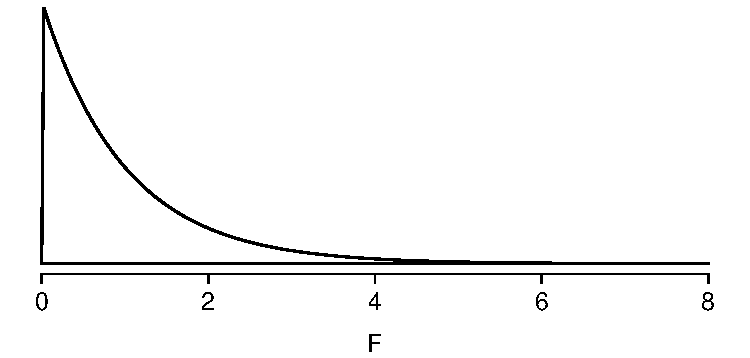
\includegraphics[width=0.65\textwidth]{ch_inference_for_means/figures/fDist2And423/fDist2And423}
\caption{An $F$ distribution with $df_1=3$ and $df_2=323$.}
\label{fDist2And423}
\end{figure}

The larger the observed variability in the sample means ($MSG$) relative to the within-group observations ($MSE$), the larger $F$ will be and the stronger the evidence against the null hypothesis. Because larger values of $F$ represent stronger evidence against the null hypothesis, we use the upper tail of the distribution to compute a p-value.

\begin{onebox}{The $F$ statistic and the $F$ test}
Analysis of variance (ANOVA) is used to test whether the mean outcome differs across 2 or more groups. ANOVA uses a test statistic $F$, which represents a standardized ratio of variability in the sample means relative to the variability within the groups. If $H_0$ is true and the model assumptions are satisfied, the statistic $F$ follows an $F$ distribution with parameters $df_{1}=k-1$ and $df_{2}=n-k$. The upper tail of the $F$ distribution is used to represent the p-value.
\end{onebox}

\begin{exercisewrap}
\begin{nexercise}
\label{describePValueAreaForFDistributionInMLBOBPExample}%
The test statistic for the baseball example is $F = \mlbF{}$. Shade the area corresponding to the p-value in Figure~\ref{fDist2And423}. \footnotemark{}
\end{nexercise}
\end{exercisewrap}
\footnotetext{\ \vspace{-4mm}\\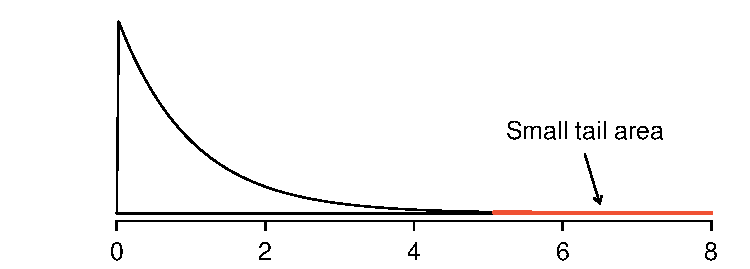
\includegraphics[height=20mm]{ch_inference_for_means/figures/fDist2And423/fDist2And423Shaded}}

\begin{examplewrap}
\begin{nexample}{The p-value corresponding to the shaded area in the solution of Guided Practice~\ref{describePValueAreaForFDistributionInMLBOBPExample} is equal to about \mlbPvalue{}. Does this provide strong evidence against the null hypothesis?}
The p-value is smaller than 0.05, indicating the evidence is strong enough to reject the null hypothesis at a significance level of 0.05. That is, the data provide strong evidence that the average on-base percentage varies by player's primary field position.
\end{nexample}
\end{examplewrap}


\subsection{Reading an ANOVA table from software}

The calculations required to perform an ANOVA by hand are tedious and prone to human error. For these reasons, it is common to use statistical software to calculate the $F$ statistic and p-value.

An ANOVA can be summarized in a table very similar to that of a regression summary, which we will see in \MultipleRegressionChapter{Chapters~\ref{linRegrForTwoVar} and~\ref{multipleAndLogisticRegression}}{Chapter~\ref{linRegrForTwoVar}}. Figure~\ref{anovaSummaryTableForOBPAgainstPosition} shows an ANOVA summary to test whether the mean of on-base percentage varies by player positions in the MLB. Many of these values should look familiar; in particular, the $F$ test statistic and p-value can be retrieved from the last columns.

\begin{figure}[ht]
\centering
\begin{tabular}{lrrrrr}
  \hline
  & Df & Sum Sq & Mean Sq & F value & Pr($>$F) \\ 
  \hline
  position & \mlbDFA{} & 0.0161 & 0.0080 & 5.0766 & 0.0066 \\ 
  Residuals & \mlbDFB{} & 0.6740 & 0.0016 &  &  \\ 

  \hline
\multicolumn{6}{r}{$s_{pooled} = 0.040$ on $df = 423$}
\end{tabular}
\caption{ANOVA summary for testing whether the average on-base percentage differs across player positions.}
\label{anovaSummaryTableForOBPAgainstPosition}
\end{figure}


\subsection{Graphical diagnostics for an ANOVA analysis}

There are three conditions we must check for an ANOVA analysis: all observations must be independent, the data in each group must be nearly normal, and the variance within each group must be approximately equal.

\begin{description}
\item[Independence.]
    If the data are a simple random sample,
    this condition is satisfied.
    For processes and experiments, carefully consider whether
    the data may be independent (e.g. no pairing).
    For example, in the MLB data, the data were not sampled.
    However, there are not obvious reasons why independence
    would not hold for most or all observations.
\item[Approximately normal.]
    As with one- and two-sample testing for means,
    the normality assumption is especially important
    when the sample size is quite small when it is
    ironically difficult to check for non-normality.
    A histogram of the observations from each group
    is shown in Figure~\ref{mlbANOVADiagNormalityGroups}.
    Since each of the groups we're considering have
    relatively large sample sizes,
    what we're looking for are major outliers.
    None are apparent, so this conditions is reasonably met.
%    there is some deviation from normality for outfielders,
%    but this isn't a substantial concern since there are
%    about 160 observations in that group and the outliers
%    are not extreme.
%    Sometimes in ANOVA there are so many groups or so few
%    observations per group that checking normality for each
%    group isn't reasonable.
%    See the footnote\footnote{First calculate the
%        \termsub{residuals}{residual} of the baseball
%        data, which are calculated by taking the observed
%        values and subtracting the corresponding group means.
%        For example, an outfielder with OBP of 0.405 would
%        have a residual of $0.405 - \bar{x}_{OF} = 0.071$.
%        Then to check the normality condition,
%        create a normal probability plot using all
%        the residuals simultaneously.}
%    for guidance on how to handle such instances.

\begin{figure}[h]
  \centering
  \Figures{}{mlbANOVA}{mlbANOVADiagNormalityGroups}
  \caption{Histograms of OBP for each field position.}
  \label{mlbANOVADiagNormalityGroups}
\end{figure}

\item[Constant variance.]
    The last assumption is that the variance in the
    groups is about equal from one group to the next.
    This assumption can be checked by examining a
    side-by-side box plot of the outcomes across the
    groups, as in Figure~\vref{mlbANOVABoxPlot}.
    In this case, the variability is similar in the
    four groups but not identical.
    We see in Table~\vref{mlbHRPerABSummaryTable}
    that the standard deviation doesn't vary much
    from one group to the next.

\index{data!MLB batting|)}

\end{description}

\begin{onebox}{Diagnostics for an ANOVA analysis}
  Independence is always important to an ANOVA analysis.
  The normality condition is very important when the sample
  sizes for each group are relatively small.
  The constant variance condition is especially important
  when the sample sizes differ between groups.
\end{onebox}


\subsection{Multiple comparisons and controlling Type~1 Error rate}
\label{multipleComparisonsAndControllingTheType1ErrorRate}

\index{significance level!multiple comparisons|(}

When we reject the null hypothesis in an ANOVA analysis, we might wonder, which of these groups have different means? To answer this question, we compare the means of each possible pair of groups. For instance, if there are three groups and there is strong evidence that there are some differences in the group means, there are three comparisons to make: group 1 to group 2, group 1 to group 3, and group 2 to group 3. These comparisons can be accomplished using a two-sample $t$-test, but we use a modified significance level and a pooled estimate of the standard deviation across groups. Usually this pooled standard deviation can be found in the ANOVA table, e.g. along the bottom of Figure~\ref{anovaSummaryTableForOBPAgainstPosition}.

\begin{examplewrap}
\begin{nexample}{Example~\vref{firstExampleForThreeStatisticsClassesAndANOVA} discussed three statistics lectures, all taught during the same semester. Figure~\ref{summaryStatisticsForClassTestData} shows summary statistics for these three courses, and a side-by-side box plot of the data is shown in Figure~\ref{classDataSBSBoxPlot}. We would like to conduct an ANOVA for these data. Do you see any deviations from the three conditions for ANOVA?}
In this case (like many others) it is difficult to check independence in a rigorous way. Instead, the best we can do is use common sense to consider reasons the assumption of independence may not hold. For instance, the independence assumption may not be reasonable if there is a star teaching assistant that only half of the students may access; such a scenario would divide a class into two subgroups. No such situations were evident for these particular data, and we believe that independence is acceptable.

The distributions in the side-by-side box plot appear to be roughly symmetric and show no noticeable outliers.

The box plots show approximately equal variability, which can be verified in Figure~\ref{summaryStatisticsForClassTestData}, supporting the constant variance assumption.
\end{nexample}
\end{examplewrap}

\begin{figure}
\centering
\begin{tabular}{lrrr}
  \hline
Class $i$	& A	& B	& C \\ 
  \hline
$n_i$		& 58	& 55	& 51 \\ 
$\bar{x}_i$	& 75.1	& 72.0	& 78.9 \\ 
$s_i$		& 13.9	& 13.8	& 13.1 \\ 
\hline
\end{tabular}
\caption{Summary statistics for the first midterm scores in three different lectures of the same course.}
\label{summaryStatisticsForClassTestData}
\end{figure}

\begin{figure}
  \centering
  \Figures{0.72}{classData}{classDataSBSBoxPlot}
  \caption{Side-by-side box plot for the first midterm
      scores in three different  lectures of the same course.}
  \label{classDataSBSBoxPlot}
\end{figure}

\begin{exercisewrap}
\begin{nexercise} \label{exerExaminingAnovaSummaryTableForMidtermData}
An ANOVA was conducted for the midterm data, and summary results are shown in Figure~\ref{anovaSummaryTableForMidtermData}. What should we conclude?\footnotemark{}
\end{nexercise}
\end{exercisewrap}
\footnotetext{The p-value of the test is 0.0330, less than the default significance level of 0.05. Therefore, we reject the null hypothesis and conclude that the difference in the average midterm scores are not due to chance.}

\begin{figure}
\centering
\begin{tabular}{lrrrrr}
  \hline
 & Df & Sum Sq & Mean Sq & F value & Pr($>$F) \\ 
  \hline
lecture & 2 & 1290.11 & 645.06 & 3.48 & 0.0330 \\ 
  Residuals & 161 & 29810.13 & 185.16 &  &  \\ 
   \hline
\multicolumn{6}{r}{$s_{pooled}=13.61$ on $df=161$}
\end{tabular}
\caption{ANOVA summary table for the midterm data.}
\label{anovaSummaryTableForMidtermData}
\end{figure}

There is strong evidence that the different means in each of the three classes is not simply due to chance. We might wonder, which of the classes are actually different? As discussed in earlier chapters, a two-sample $t$-test could be used to test for differences in each possible pair of groups. However, one pitfall was discussed in Example~\vref{multipleComparisonExampleThatIncludesDiscussionOfClassrooms}: when we run so many tests, the Type~1 Error rate increases. This issue is resolved by using a modified significance level.

\begin{onebox}{Multiple comparisons and the Bonferroni correction for $\alpha$}
The scenario of testing many pairs of groups is called \term{multiple comparisons}. The \term{Bonferroni correction} suggests that a more stringent significance level is more appropriate for these tests:
\begin{align*}
\alpha^* = \alpha / K
\end{align*}
where $K$ is the number of comparisons being considered (formally or informally). If there are $k$ groups, then usually all possible pairs are compared and $K=\frac{k(k-1)}{2}$.
\end{onebox}

\begin{examplewrap}
\begin{nexample}{In Guided Practice~\ref{exerExaminingAnovaSummaryTableForMidtermData}, you found strong evidence of differences in the average midterm grades between the three lectures. Complete the three possible pairwise comparisons using the Bonferroni correction and report any differences.} \label{multipleComparisonsOfThreeStatClasses}
We use a modified significance level of $\alpha^* = 0.05/3 = 0.0167$. Additionally, we use the pooled estimate of the standard deviation: $s_{pooled}=13.61$ on $df=161$, which is provided in the ANOVA summary table.

Lecture A versus Lecture B: The estimated difference and
standard error are, respectively,
\begin{align*}
\bar{x}_A - \bar{x}_{B} &= 75.1 - 72 = 3.1
	&SE = \sqrt{\frac{13.61^2}{58} + \frac{13.61^2}{55}} &= 2.56
\end{align*}
(See Section~\vref{pooledStandardDeviations} for additional
details.)
This results in a T-score of 1.21 on $df = 161$
(we use the $df$ associated with $s_{pooled}$).
Statistical software was used to precisely identify the two-sided
p-value since the modified significance level of 0.0167 is not
found in the $t$-table.
The p-value (0.228) is larger than $\alpha^*=0.0167$,
so there is not strong evidence of a difference in the means
of lectures A and~B.

Lecture A versus Lecture C: The estimated difference and standard error are 3.8 and 2.61, respectively. This results in a $T$ score of 1.46 on $df = 161$ and a two-sided p-value of 0.1462. This p-value is larger than $\alpha^*$, so there is not strong evidence of a difference in the means of lectures A and C.

Lecture B versus Lecture C: The estimated difference and standard error are 6.9 and 2.65, respectively. This results in a $T$ score of 2.60 on $df = 161$ and a two-sided p-value of 0.0102. This p-value is smaller than $\alpha^*$. Here we find strong evidence of a difference in the means of lectures B and C.
\end{nexample}
\end{examplewrap}

We might summarize the findings of the analysis from Example~\ref{multipleComparisonsOfThreeStatClasses} using the following notation:
\begin{align*}
\mu_A &\stackrel{?}{=} \mu_B
	&\mu_A &\stackrel{?}{=} \mu_C
	&\mu_B &\neq \mu_C
\end{align*}
The midterm mean in lecture A is not statistically distinguishable from those of lectures B or C. However, there is strong evidence that lectures B and C are different. In the first two pairwise comparisons, we did not have sufficient evidence to reject the null hypothesis. Recall that failing to reject $H_0$ does not imply $H_0$ is true.

\begin{onebox}{Reject $\mathbf{H_0}$ with ANOVA
    but find no group differences}
  It is possible to reject the null hypothesis using ANOVA
  and then to not subsequently identify differences in the
  pairwise comparisons.
  However, \emph{this does not invalidate the ANOVA conclusion}.
  It only means we have not been able to successfully identify
  which specific groups differ in their means.
\end{onebox}

The ANOVA procedure examines the big picture: it considers all groups simultaneously to decipher whether there is evidence that some difference exists. Even if the test indicates that there is strong evidence of differences in group means, identifying with high confidence a specific difference as statistically significant is more difficult.

Consider the following analogy: we observe a Wall Street firm that makes large quantities of money based on predicting mergers. Mergers are generally difficult to predict, and if the prediction success rate is extremely high, that may be considered sufficiently strong evidence to warrant investigation by the Securities and Exchange Commission (SEC). While the SEC may be quite certain that there is insider trading taking place at the firm, the evidence against any single trader may not be very strong. It is only when the SEC considers all the data that they identify the pattern. This is effectively the strategy of ANOVA: stand back and consider all the groups simultaneously.

\index{significance level!multiple comparisons|)}
\index{analysis of variance (ANOVA)|)}

